%%%%%%%%%%%%%%%%%
% From Template %
%%%%%%%%%%%%%%%%%

\documentclass[%
class=scrreprt,
chapterprefix=false,%
open=right,%
twoside=false,%
paper=a4,%
logofile={Logo\_zentral\_farbig\_EN.png},%
thesistype=master,%
UKenglish,%
]{se2thesis}
\listfiles
\usepackage[ngerman,main=UKenglish]{babel}
\usepackage{blindtext}
\usepackage[%
csquotes=true,%
booktabs=true,%
siunitx=true,%
minted=true,%
selnolig=true,%
widowcontrol=false,%
microtype=true,%
% biblatex=true,%
cleveref=true,%
]{se2packages}

% Own change (from Lisa)
% Changing citeauthor to use et el.
\usepackage[maxcitenames=2,backend=biber]{biblatex}
% End own change

\begin{filecontents}{\jobname.bib}
@article{linaker2015guidelines,
	author = {Linåker, Johan and Sulaman, Sardar and Host, Martin and de Mello, Rafael},
	pages = {},
	title = {Guidelines for Conducting Surveys in Software Engineering},
	year = {2015}
}

@article{boehm2001defect,
	author = {Boehm, Barry and Basili, Victor R},
	journal = {Computer},
	number = {1},
	pages = {135--137},
	title = {Defect reduction top 10 list},
	volume = {34},
	year = {2001}
}

@article{buse2009learning,
	author = {Buse, Raymond PL and Weimer, Westley R},
	journal = {IEEE Transactions on software engineering},
	number = {4},
	pages = {546--558},
	publisher = {IEEE},
	title = {Learning a metric for code readability},
	volume = {36},
	year = {2009}
}

@inproceedings{aggarwal2002integrated,
	author = {Aggarwal, Krishan K and Singh, Yogesh and Chhabra, Jitender Kumar},
	booktitle = {Annual Reliability and Maintainability Symposium. 2002 Proceedings (Cat. No. 02CH37318)},
	organization = {IEEE},
	pages = {235--241},
	title = {An integrated measure of software maintainability},
	year = {2002}
}

@inproceedings{fakhoury2019improving,
	author = {Fakhoury, Sarah and Roy, Devjeet and Hassan, Adnan and Arnaoudova, Vernera},
	booktitle = {2019 IEEE/ACM 27th International Conference on Program Comprehension (ICPC)},
	organization = {IEEE},
	pages = {2--12},
	title = {Improving source code readability: Theory and practice},
	year = {2019}
}

@article{scalabrino2018comprehensive,
	author = {Scalabrino, Simone and Linares-V{\'a}squez, Mario and Oliveto, Rocco and Poshyvanyk, Denys},
	journal = {Journal of Software: Evolution and Process},
	number = {6},
	pages = {e1958},
	publisher = {Wiley Online Library},
	title = {A comprehensive model for code readability},
	volume = {30},
	year = {2018}
}

@inproceedings{posnett2011simpler,
	author = {Posnett, Daryl and Hindle, Abram and Devanbu, Premkumar},
	booktitle = {Proceedings of the 8th working conference on mining software repositories},
	pages = {73--82},
	title = {A simpler model of software readability},
	year = {2011}
}

@inproceedings{dorn2012general,
	author = {Jonathan Dorn},
	title = {A General Software Readability Model},
	year = {2012}
}

@inproceedings{scalabrino2017automatically,
	author = {Scalabrino, Simone and Bavota, Gabriele and Vendome, Christopher and Linares-V{\'a}squez, Mario and Poshyvanyk, Denys and Oliveto, Rocco},
	booktitle = {2017 32nd IEEE/ACM International Conference on Automated Software Engineering (ASE)},
	organization = {IEEE},
	pages = {417--427},
	title = {Automatically assessing code understandability: How far are we?},
	year = {2017}
}

@inproceedings{daka2015modeling,
	author = {Daka, Ermira and Campos, Jos{\'e} and Fraser, Gordon and Dorn, Jonathan and Weimer, Westley},
	booktitle = {Proceedings of the 2015 10th Joint Meeting on Foundations of Software Engineering},
	pages = {107--118},
	title = {Modeling readability to improve unit tests},
	year = {2015}
}

@article{mi2022towards,
	author = {Mi, Qing and Hao, Yiqun and Ou, Liwei and Ma, Wei},
	journal = {Journal of Systems and Software},
	pages = {111454},
	publisher = {Elsevier},
	title = {Towards using visual, semantic and structural features to improve code readability classification},
	volume = {193},
	year = {2022}
}

@inproceedings{mi2018gamification,
	author = {Mi, Qing and Keung, Jacky and Mei, Xiupei and Xiao, Yan and Chan, WK},
	booktitle = {2018 International Symposium on Educational Technology (ISET)},
	organization = {IEEE},
	pages = {250--254},
	title = {A gamification technique for motivating students to learn code readability in software engineering},
	year = {2018}
}

@article{mi2018improving,
	author = {Mi, Qing and Keung, Jacky and Xiao, Yan and Mensah, Solomon and Gao, Yujin},
	journal = {Information and Software Technology},
	pages = {60--71},
	publisher = {Elsevier},
	title = {Improving code readability classification using convolutional neural networks},
	volume = {104},
	year = {2018}
}

@book{brooks1987no,
	author = {Brooks, Frederick and Kugler, H},
	publisher = {April},
	title = {No silver bullet},
	year = {1987}
}

@article{loriot2022styler,
	author = {Loriot, Benjamin and Madeiral, Fernanda and Monperrus, Martin},
	journal = {Empirical Software Engineering},
	number = {6},
	pages = {149},
	publisher = {Springer},
	title = {Styler: learning formatting conventions to repair Checkstyle violations},
	volume = {27},
	year = {2022}
}

@inproceedings{yasunaga2020graph,
	author = {Michihiro Yasunaga and
		Percy Liang},
	bibsource = {dblp computer science bibliography, https://dblp.org},
	biburl = {https://dblp.org/rec/conf/icml/YasunagaL20.bib},
	booktitle = {Proceedings of the 37th International Conference on Machine Learning,
		{ICML} 2020, 13-18 July 2020, Virtual Event},
	pages = {10799--10808},
	publisher = {{PMLR}},
	series = {Proceedings of Machine Learning Research},
	timestamp = {Tue, 15 Dec 2020 00:00:00 +0100},
	title = {Graph-based, Self-Supervised Program Repair from Diagnostic Feedback},
	url = {http://proceedings.mlr.press/v119/yasunaga20a.html},
	volume = {119},
	year = {2020}
}

@inproceedings{xu2019method,
	author = {Xu, Sihan and Zhang, Sen and Wang, Weijing and Cao, Xinya and Guo, Chenkai and Xu, Jing},
	booktitle = {Proceedings of the 2019 ACM SIGPLAN workshop on partial evaluation and program manipulation},
	pages = {10--21},
	title = {Method name suggestion with hierarchical attention networks},
	year = {2019}
}

@inproceedings{allamanis2016convolutional,
	author = {Miltiadis Allamanis and
		Hao Peng and
		Charles Sutton},
	bibsource = {dblp computer science bibliography, https://dblp.org},
	biburl = {https://dblp.org/rec/conf/icml/AllamanisPS16.bib},
	booktitle = {Proceedings of the 33nd International Conference on Machine Learning,
		{ICML} 2016, New York City, NY, USA, June 19-24, 2016},
	editor = {Maria{-}Florina Balcan and
		Kilian Q. Weinberger},
	pages = {2091--2100},
	publisher = {JMLR.org},
	series = {{JMLR} Workshop and Conference Proceedings},
	timestamp = {Mon, 12 Oct 2020 01:00:00 +0200},
	title = {A Convolutional Attention Network for Extreme Summarization of Source
		Code},
	url = {http://proceedings.mlr.press/v48/allamanis16.html},
	volume = {48},
	year = {2016}
}

@article{hestness2017deep,
	author = {Hestness, Joel and Narang, Sharan and Ardalani, Newsha and Diamos, Gregory and Jun, Heewoo and Kianinejad, Hassan and Patwary, Md Mostofa Ali and Yang, Yang and Zhou, Yanqi},
	journal = {ArXiv preprint},
	title = {Deep learning scaling is predictable, empirically},
	url = {https://arxiv.org/abs/1712.00409},
	volume = {abs/1712.00409},
	year = {2017}
}

@inproceedings{liu2019learning,
	author = {Liu, Kui and Kim, Dongsun and Bissyand{\'e}, Tegawend{\'e} F and Kim, Taeyoung and Kim, Kisub and Koyuncu, Anil and Kim, Suntae and Le Traon, Yves},
	booktitle = {2019 IEEE/ACM 41st International Conference on Software Engineering (ICSE)},
	organization = {IEEE},
	pages = {1--12},
	title = {Learning to spot and refactor inconsistent method names},
	year = {2019}
}

@article{deimel1985uses,
	author = {Deimel Jr, Lionel E},
	journal = {ACM SIGCSE Bulletin},
	number = {2},
	pages = {5--14},
	publisher = {ACM New York, NY, USA},
	title = {The uses of program reading},
	volume = {17},
	year = {1985}
}

@inproceedings{raymond1991reading,
	author = {Raymond, Darrell R},
	booktitle = {CASCON},
	pages = {3--16},
	title = {Reading source code.},
	volume = {91},
	year = {1991}
}

@article{rugaber2000use,
	author = {Rugaber, Spencer},
	journal = {Annals of Software Engineering},
	number = {1-4},
	pages = {143--192},
	publisher = {Springer},
	title = {The use of domain knowledge in program understanding},
	volume = {9},
	year = {2000}
}

@article{likert1932technique,
	author = {Likert, Rensis},
	journal = {Archives of psychology},
	title = {A technique for the measurement of attitudes.},
	year = {1932}
}

@inproceedings{wyrich2019towards,
	author = {Wyrich, Marvin and Bogner, Justus},
	booktitle = {2019 IEEE/ACM 1st international workshop on bots in software engineering (BotSE)},
	organization = {IEEE},
	pages = {24--28},
	title = {Towards an autonomous bot for automatic source code refactoring},
	year = {2019}
}

@article{pawlak2016spoon,
	author = {Pawlak, Renaud and Monperrus, Martin and Petitprez, Nicolas and Noguera, Carlos and Seinturier, Lionel},
	journal = {Software: Practice and Experience},
	number = {9},
	pages = {1155--1179},
	publisher = {Wiley Online Library},
	title = {Spoon: A library for implementing analyses and transformations of java source code},
	volume = {46},
	year = {2016}
}

@article{someoliayi2022sorald,
	author = {Someoliayi, Khashayar Etemadi and Harrand, Nicolas Yves Maurice and Larsen, Simon and Adzemovic, Haris and Phu, Henry Luong and Verma, Ashutosh and Madeiral, Fernanda and Wikstrom, Douglas and Monperrus, Martin},
	journal = {IEEE Transactions on Dependable and Secure Computing},
	publisher = {IEEE},
	title = {Sorald: Automatic Patch Suggestions for SonarQube Static Analysis Violations},
	year = {2022}
}

@inproceedings{allamanis2015suggesting,
	author = {Allamanis, Miltiadis and Barr, Earl T and Bird, Christian and Sutton, Charles},
	booktitle = {Proceedings of the 2015 10th joint meeting on foundations of software engineering},
	pages = {38--49},
	title = {Suggesting accurate method and class names},
	year = {2015}
}

@article{alon2019code2vec,
	author = {Alon, Uri and Zilberstein, Meital and Levy, Omer and Yahav, Eran},
	journal = {Proceedings of the ACM on Programming Languages},
	number = {POPL},
	pages = {1--29},
	publisher = {ACM New York, NY, USA},
	title = {code2vec: Learning distributed representations of code},
	volume = {3},
	year = {2019}
}

@article{chicco2020advantages,
	author = {Chicco, Davide and Jurman, Giuseppe},
	journal = {BMC genomics},
	number = {1},
	pages = {1--13},
	publisher = {BioMed Central},
	title = {The advantages of the Matthews correlation coefficient (MCC) over F1 score and accuracy in binary classification evaluation},
	volume = {21},
	year = {2020}
}

@article{dubay2004principles,
	author = {DuBay, William H},
	journal = {Online Submission},
	publisher = {ERIC},
	title = {The principles of readability.},
	year = {2004}
}

@book{klare1964measurement,
	author = {Klare, George R.},
	date = {1963},
	keywords = {Bibliographies, Bibliography, Readability (Literary style)},
	location = {Ames},
	pagetotal = {328},
	publisher = {Iowa State University Press},
	title = {The measurement of readability}
}

@article{tashtoush2013impact,
	author = {Tashtoush, Yahya and Odat, Zeinab and Alsmadi, Izzat M and Yatim, Maryan},
	title = {Impact of programming features on code readability},
	year = {2013}
}

@inproceedings{sedano2016code,
	author = {Sedano, Todd},
	booktitle = {2016 IEEE 29th International conference on software engineering education and training (CSEET)},
	organization = {IEEE},
	pages = {111--117},
	title = {Code readability testing, an empirical study},
	year = {2016}
}

@inproceedings{oliveira2020evaluating,
	author = {Oliveira, Delano and Bruno, Reydne and Madeiral, Fernanda and Castor, Fernando},
	booktitle = {2020 IEEE International Conference on Software Maintenance and Evolution (ICSME)},
	organization = {IEEE},
	pages = {348--359},
	title = {Evaluating code readability and legibility: An examination of human-centric studies},
	year = {2020}
}

@article{mi2023graph,
	author = {Mi, Qing and Zhan, Yi and Weng, Han and Bao, Qinghang and Cui, Longjie and Ma, Wei},
	journal = {Empirical Software Engineering},
	number = {4},
	pages = {87},
	publisher = {Springer},
	title = {A graph-based code representation method to improve code readability classification},
	volume = {28},
	year = {2023}
}

@article{mi2021effectiveness,
	author = {Mi, Qing and Xiao, Yan and Cai, Zhi and Jia, Xibin},
	journal = {Information and Software Technology},
	pages = {106378},
	publisher = {Elsevier},
	title = {The effectiveness of data augmentation in code readability classification},
	volume = {129},
	year = {2021}
}

@book{martin2009clean,
	author = {Martin, Robert C},
	publisher = {Pearson Education},
	title = {Clean code: a handbook of agile software craftsmanship},
	year = {2009}
}

@book{wilson2007beautiful,
	author = {Wilson, Greg and Oram, Andy},
	publisher = {" O'Reilly Media, Inc."},
	title = {Beautiful code: Leading programmers explain how they think},
	year = {2007}
}

@book{beck2007implementation,
	author = {Beck, Kent},
	publisher = {Pearson Education},
	title = {Implementation patterns},
	year = {2007}
}

@article{alawad2019empirical,
	author = {Alawad, Duaa and Panta, Manisha and Zibran, Minhaz and Islam, Md Rakibul},
	journal = {ArXiv preprint},
	title = {An empirical study of the relationships between code readability and software complexity},
	url = {https://arxiv.org/abs/1909.01760},
	volume = {abs/1909.01760},
	year = {2019}
}

@inproceedings{mannan2018towards,
	author = {Mannan, Umme Ayda and Ahmed, Iftekhar and Sarma, Anita},
	booktitle = {Proceedings of the 4th ACM SIGSOFT International Workshop on NLP for Software Engineering},
	pages = {18--21},
	title = {Towards understanding code readability and its impact on design quality},
	year = {2018}
}

@inproceedings{johnson2019empirical,
	author = {Johnson, John and Lubo, Sergio and Yedla, Nishitha and Aponte, Jairo and Sharif, Bonita},
	booktitle = {2019 IEEE International conference on software maintenance and evolution (ICSME)},
	organization = {IEEE},
	pages = {513--523},
	title = {An empirical study assessing source code readability in comprehension},
	year = {2019}
}

@article{xia2017measuring,
	author = {Xia, Xin and Bao, Lingfeng and Lo, David and Xing, Zhenchang and Hassan, Ahmed E and Li, Shanping},
	journal = {IEEE Transactions on Software Engineering},
	number = {10},
	pages = {951--976},
	publisher = {IEEE},
	title = {Measuring program comprehension: A large-scale field study with professionals},
	volume = {44},
	year = {2017}
}

@article{segedinac2024assessing,
	author = {Segedinac, Milan and Savi{\'c}, Goran and Zeljkovi{\'c}, Ivana and Slivka, Jelena and Konjovi{\'c}, Zora},
	journal = {Computer Applications in Engineering Education},
	number = {1},
	pages = {e22685},
	publisher = {Wiley Online Library},
	title = {Assessing code readability in Python programming courses using eye-tracking},
	volume = {32},
	year = {2024}
}

@article{ribeiro2018attributes,
	author = {Ribeiro, Talita Vieira and Travassos, Guilherme Horta},
	journal = {CLEI Electronic Journal},
	number = {1},
	pages = {5--1},
	title = {Attributes influencing the reading and comprehension of source code--discussing contradictory evidence},
	volume = {21},
	year = {2018}
}

@inproceedings{mi2018inception,
	author = {Mi, Qing and Keung, Jacky and Xiao, Yan and Mensah, Solomon and Mei, Xiupei},
	booktitle = {Proceedings of the 22nd International Conference on Evaluation and Assessment in Software Engineering 2018},
	pages = {139--144},
	title = {An inception architecture-based model for improving code readability classification},
	year = {2018}
}

@inproceedings{sharma2020egan,
	author = {Sharma, Shashank and Srivastava, Sumit},
	booktitle = {2020 International Conference on Computation, Automation and Knowledge Management (ICCAKM)},
	organization = {IEEE},
	pages = {312--316},
	title = {EGAN: An Effective Code Readability Classification using Ensemble Generative Adversarial Networks},
	year = {2020}
}

@article{choi2020metric,
	author = {Choi, Sangchul and Park, Sooyong and others},
	journal = {Tehni{\v{c}}ki vjesnik},
	number = {1},
	pages = {221--228},
	publisher = {Faculty of Mechanical Engineering in Slavonski Brod; Faculty of Electrical~…},
	title = {Metric and tool support for instant feedback of source code readability},
	volume = {27},
	year = {2020}
}

@inproceedings{mi2022enhanced,
	author = {Mi, Qing and Hao, Yiqun and Wu, Maran and Ou, Liwei},
	booktitle = {International conference on software engineering and knowledge engineering},
	title = {An enhanced data augmentation approach to support multi-class code readability classification},
	year = {2022}
}

@inproceedings{vitale2023using,
	author = {Vitale, Antonio and Piantadosi, Valentina and Scalabrino, Simone and Oliveto, Rocco},
	booktitle = {2023 38th IEEE/ACM International Conference on Automated Software Engineering (ASE)},
	organization = {IEEE},
	pages = {573--584},
	title = {Using Deep Learning to Automatically Improve Code Readability},
	year = {2023}
}

@inproceedings{mi2022rank,
	author = {Mi, Qing},
	booktitle = {Proceedings of the 37th IEEE/ACM International Conference on Automated Software Engineering},
	pages = {1--2},
	title = {Rank Learning-Based Code Readability Assessment with Siamese Neural Networks},
	year = {2022}
}

@article{mi2023makes,
	author = {Mi, Qing and Chen, Mingjie and Cai, Zhi and Jia, Xibin},
	journal = {Software: Practice and Experience},
	number = {6},
	pages = {1391--1409},
	publisher = {Wiley Online Library},
	title = {What makes a readable code? A causal analysis method},
	volume = {53},
	year = {2023}
}

@inproceedings{buse2008metric,
	title={A metric for software readability},
	author={Buse, Raymond PL and Weimer, Westley R},
	booktitle={Proceedings of the 2008 international symposium on Software testing and analysis},
	pages={121--130},
	year={2008}
}

% TODO: Use scalabrino2018comprehensive instead?
@inproceedings{scalabrino2016improving,
	title={Improving code readability models with textual features},
	author={Scalabrino, Simone and Linares-Vasquez, Mario and Poshyvanyk, Denys and Oliveto, Rocco},
	booktitle={2016 IEEE 24th International Conference on Program Comprehension (ICPC)},
	pages={1--10},
	year={2016},
	organization={IEEE}
}

@article{mullner2013fastcluster,
	title={fastcluster: Fast hierarchical, agglomerative clustering routines for R and Python},
	author={M{\"u}llner, Daniel},
	journal={Journal of Statistical Software},
	volume={53},
	pages={1--18},
	year={2013}
}

\end{filecontents}
\addbibresource{\jobname.bib}

\usepackage{hyperref}

\author{Lukas Krodinger}
\title{Advancing Code Readability: Mined \& Modified Code for Dataset Generation}
\degreeprogramme{M.Sc. Computer Science}
\matrnumber{89801}
\supervisor{Prof. Dr. Gordon Fraser}
%\external{Prof.~John Doe,~PhD}
\advisor{Lisa Griebl}
\department{Faculty of Computer Science and Mathematics}
\institute{Chair of Software Engineering II}
\location{Passau}


%%%%%%%%%%%%%%%%%%%%%%
% Installed Packages %
%%%%%%%%%%%%%%%%%%%%%%
% For java code embeddings
\usepackage{color}
\definecolor{dkgreen}{rgb}{0,0.6,0}
\definecolor{gray}{rgb}{0.5,0.5,0.5}
\definecolor{mauve}{rgb}{0.58,0,0.82}

\usepackage{listings}
\lstset{frame=tb,
	language=Java,
	aboveskip=3mm,
	belowskip=3mm,
	showstringspaces=false,
	columns=flexible,
	basicstyle={\small\ttfamily},
	showstringspaces=true,
	numbers=none,
	numberstyle=\tiny\color{gray},
	keywordstyle=\color{blue},
	commentstyle=\color{dkgreen},
	stringstyle=\color{mauve},
	breaklines=true,
	breakatwhitespace=true,
	tabsize=3
}

% Start counting of chapters with 1
\usepackage{chngcntr}
\counterwithout{chapter}{section}
\counterwithin{chapter}{part}
\renewcommand{\thesection}{\arabic{section}}
\renewcommand{\thechapter}{\arabic{chapter}.0}

% Footnotes
\newcounter{urlfootnote}
\newcommand{\onecurl}[2]{%
	\stepcounter{urlfootnote}%
	\expandafter\def\csname urlfootnote:#1\endcsname{\theurlfootnote}%
	\footnote{\label{url:#1}\url{#1}, accessed: #2}%
}
\usepackage{etoolbox}
\newcommand{\curl}[2]{%
	\ifcsdef{urlfootnote:#1}{%
		\textsuperscript{\ref{url:#1}}%
	}{%
		\onecurl{#1}{#2}%
	}%
}

% Indentation of "Assumption 1" etc. in enumerate
\usepackage{enumitem}

% Nice skips between paragraphs
\usepackage{parskip} 

% Skips at \_ within table
\usepackage{seqsplit}

% Definitions
\theoremstyle{definition}
\newtheorem{definition}{Definition}[section]

\begin{document}
	
	\frontmatter
	
	\maketitle
	
	\begin{abstract}
		% TODO: Rework once work is done
		This work presents an innovative method for generating datasets intended for code readability classification in the context of a master's thesis. We offer a comprehensive overview of code readability, delving into existing classifiers that consider both manually crafted and automatically extracted code readability features. Furthermore, we summarize existing datasets of manually annotated Java code snippets.
		
		The core contribution of this work lies in the introduction of an automatic data generation technique, alongside a dataset produced using this methodology. Our approach relies on the extraction and modification of code snippets sourced from public GitHub repositories. Notably, our dataset significantly surpasses the scale of any previously available dataset designed for readability classification.
		
		To evaluate the newly generated dataset, we conducted a user survey and train a state of the art code readability classification model, both with and without the integration of the new dataset. This analysis aims to assess the quality of our new dataset and the effectiveness of the generation approach employed.

	\end{abstract}
	
	\mainmatter
	
	\tableofcontents
	
\section{Introduction} \label{Introduction}
	In the realm of software development, the significance of code readability cannot be overstated. Together with understandability, it serves as the foundation for efficient collaboration, comprehension, and maintenance of software systems~\cite{posnett2011simpler, aggarwal2002integrated}. 
	Maintenance alone will consume over 70\% of the total lifecycle cost of a software product and for maintenance, the most time-consuming act is reading code~\cite{buse2009learning, deimel1985uses, rugaber2000use, boehm2001defect}.
	Therefore, it is important to ensure a high readability of code. In order to archive this, we need to measure readability.
	
	In the last years, researchers have proposed several metrics and models for assessing code readability with an accuracy of up to 81.8\%~\cite{buse2009learning, posnett2011simpler, dorn2012general, daka2015modeling}. In recent years, deep learning based models are able to achieve an accuracy of up to 85.3\%~\cite{mi2018improving, mi2022towards}.
	However, these models do not capture what developers think of readability improvements~\cite{fakhoury2019improving}. This suggests that there is room for improvement in readability classification of source code. 
	
	% TODO: Add Sections ref
	% Background and related work
	In the following sections we will clarify what source code readability is. We will summarize background knowledge for both classical and deep learning based classification approaches. We will have a look at related work.
	
	% Dataset generation approach
	In section TODO we will explain our new dataset generation approach in detail. We will SUBSECTIONS
	
	% Readability Classification model
	After introducing our new dataset we will evaluate it based on a user study and a state of the art readability classification model in section TODO. Based on the dataset, the user study and the model we will propose our research questions.
	
	% Evaluation
	We will then answer our research questions based on results of the survey and model performance in section TODO.
	
	% Discussion
	We will show possible threads to the dataset generation approach and our evaluation and discuss them in section TODO.
	
	% Conclusion
	In the last section we summarize our work, draw conclusions from it and propose future work.
	
\section{Background and related work} \label{Background and related work}
	In the following subsections you find an overview of the background and related work on code readability and our approach to dataset creation.
	
\subsection{Code Readability} \label{Readability}
		
	% Importance	
	In the domain of software development, the importance of code readability cannot be emphasized enough. Alongside understandability, it forms the basis for effective collaboration, comprehension, and maintenance of software systems~\cite{posnett2011simpler, aggarwal2002integrated}.
	
	It is a critical aspect of software quality, significantly influencing the maintainability, reusability, portability, and reliability of the source code \cite{alawad2019empirical, sedano2016code}. Poorly readable code increases the risk of introducing bugs \cite{mannan2018towards, scalabrino2018comprehensive} and can lead to higher costs during subsequent software maintenance and development \cite{johnson2019empirical}. On the other hand, readable code allows developers to identify and rectify bugs more easily \cite{mi2023graph}.
	
	Recent studies indicate that developers spend nearly 58\% of their time reading and comprehending source code~\cite{buse2009learning, deimel1985uses, rugaber2000use, boehm2001defect, tashtoush2013impact, sedano2016code, xia2017measuring}.
	%	In the field of software development, a major focus continues to be on code readability and its profound impact on these aspects, as confirmed by numerous studies~\cite{deimel1985uses, rugaber2000use, boehm2001defect, aggarwal2002integrated, posnett2011simpler, buse2009learning, tashtoush2013impact, sedano2016code, xia2017measuring, mannan2018towards, scalabrino2018comprehensive, alawad2019empirical, johnson2019empirical, mi2023graph}.
	Therefore, it is important to ensure a high readability of code. In order to archive this, we need to define and measure code readability.
%	However, there are various definitions in the literature:
	
	% Readability in general
	%\citeauthor{klare1964measurement} defines readability in general as “the ease of understanding or comprehension due to the style of writing.” 

	% Readability in general
	%https://files.eric.ed.gov/fulltext/ED490073.pdf
	%	 This definition focuses on writing
	%	style as separate from issues such as content, coherence, and organization. In a
	%	similar manner, Gretchen Hargis and her colleagues at IBM (1998) state that
	%	readability, the “ease of reading words and sentences,” is an attribute of clarity.
	%	The creator of the SMOG readability formula G. Harry McLaughlin (1969)
	%	defines readability as: “the degree to which a given class of people find certain
	%	reading matter compelling and comprehensible.” This definition stresses the
	%	interaction between the text and a class of readers of known characteristics such
	%	as reading skill, prior knowledge, and motivation.
	%	Edgar Dale and Jeanne Chall’s (1949) definition may be the most
	%	comprehensive: “The sum total (including all the interactions) of all those
	%	elements within a given piece of printed material that affect the success a group
	%	of readers have with it. The success is the extent to which they understand it,
	%	read it at an optimal speed, and find it interesting.” 
	%	\cite{dubay2004principles}
	
	% Definiton
	\citeauthor{buse2009learning} provides one of the first definitions: "We define readability as a human judgment of how easy a
	text is to understand."

	% Definition
	\citeauthor{tashtoush2013impact} combines numerous other aspects from various definitions. According to them code readability can be measured by looking at the following aspects \cite{tashtoush2013impact}:
	\begin{itemize}
		\item Ratio between lines of code and number of commented lines
		\item Writing to people not to computers
		\item Making a code locally understandable without searching for declarations and definitions
		\item Average number of right answers to a series of questions about a program in a given length of time
	\end{itemize}
	
	% Definition
	Recent definitions of code readability are shorter, trying to focus on the key aspects. \citeauthor{oliveira2020evaluating} defines readability as "what makes a program easier or harder to read and apprehend by developers" \cite{oliveira2020evaluating}.
			
	% Definition
	Also \citeauthor{mi2021effectiveness} summarizes code readability as "a human judgment of how easy a piece of
	source code is to understand" \cite{mi2021effectiveness}. This comes close to the definition of \citeauthor{buse2009learning}~\cite{buse2009learning}.
	
	% Related terms	
	There are various related terms to readability: Understandability, usability, reusability, complexity, and maintainability \cite{tashtoush2013impact}~\cite{tashtoush2013impact}. Among those especially complexity and understandability are closely related to readability.
	
	Readability is not the same as complexity. Complexity is an “essential” property of software that arises
	from system requirements, while readability is an “accidental” property that is not determined by the problem statement~\cite{buse2009learning, brooks1987no}.
	
	Readability is neither the same as understandability, as the key aspects of understandability are \cite{scalabrino2018comprehensive, martin2009clean, wilson2007beautiful, beck2007implementation}:
	\begin{itemize}
		\item Complexity
		\item Usage of design concepts
		\item Formatting
		\item Source code lexicon
		\item Visual aspects (e.g., syntax highlighting)
	\end{itemize}
	
	\citeauthor{posnett2011simpler} states that readability is the syntactic aspect of processing code, while understandability is the semantic aspect \cite{posnett2011simpler}.
	
	Based on \citeauthor{posnett2011simpler}, \citeauthor{scalabrino2018comprehensive} writes about readability: "Readability measures the effort of the developer to access the information contained in the code, while understandability measures the complexity of such information" \cite{scalabrino2018comprehensive, posnett2011simpler}.
	
	%	Readability is a human judgment of how easy a program source code is to read and comprehend \cite{buse2008metric, sedano2016code}. It is concerned with the syntactic aspects of code, such as the use of meaningful variable names, consistent formatting, and clear commenting.
	%	
	%	Understandability is the ability to grasp the meaning of a program source code and how it works \cite{oliveira2020evaluating, posnett2011simpler}. It is concerned with the semantic aspects of code, such as the underlying logic and the use of design patterns.
	
	For example, a developer can find a piece of code readable but still difficult to understand. Recent research gives evidence that there is no correlation between understandability and readability~\cite{scalabrino2017automatically}.	
	
	
	% However, \citeauthor{scalabrino2018comprehensive} also states, that "code readability remains to be a very subjective concept".
		
	%	
	%	For now we stick with the definition of BUSE and WEIMER which also \citeauthor{mi2023graph} sticks with:
	%	Code readability is defined as a measure of how easily developers can read and understand
	%	the source code (Buse and Weimer 2010; Lee et al 2013)
	%	% TODO: Continue

	Comparing the definitions of code readability in literature we can see, that there are some common aspects in most definitions. These are:
	\begin{itemize}
		\item Ease/complexity of understanding/comprehension/apprehension
		\item Human judgment/assessment
		\item Effort of the process of reading (differentiation to understandability)
	\end{itemize}
	Based on this, we come up with the following definition: 
	\begin{definition}[Code readability]
		Code readability is the human assessment of the effort required to read and understand code.
	\end{definition}

	% TODO: Update citations
	In the last years, researchers have proposed several metrics and models for assessing code readability with an accuracy of up to 81.8\%~\cite{buse2009learning, posnett2011simpler, dorn2012general, daka2015modeling}. In recent years, deep learning based models are able to achieve an accuracy of to 85.3\%~\cite{mi2018improving, mi2022towards} on available datasets. By using data augmentation the score can be improved even further to 87.3\% \cite{mi2021effectiveness}.
%	However, these models do not capture what developers think of readability improvements~\cite{fakhoury2019improving}. This suggests that there is room for improvement in readability classification of source code.
	Examining these works more closely in the following, we delve into their intricacies.
	
%	% Importance
%	In software engineering, the terms readability, legibility, understandability, and comprehensibility have overlapping meanings. For example, Buse and Weimer [22] define “readability
%	as a human judgment of how easy a text is to understand”.
%	In a similar vein, Almeida et al. [23] affirm that “legibility is
%	fundamental to code maintenance; if source code is written
%	in a complex way, understanding it will require much more
%	effort”. In addition, Lin and Wu [24] state that ““Software
%	understandability” determines whether a system can be understood by other individuals easily, or whether artifacts of
%	one system can be easily understood by other individuals”.
%	Xia et al. [25] treat comprehension and understanding as
%	synonyms, expressing that “Program comprehension (aka.,
%	program understanding, or source code comprehension) is a
%	process where developers actively acquire knowledge about a
%	software system by exploring and searching software artifacts,
%	and reading relevant source code and/or documentation”.\cite{oliveira2020evaluating}
%	
%	% Importance
%	Software developers read code all the time. The very first step in each software evolution and
%	maintenance task is to carefully read and understand the code; this step needs to be done even
%	when the maintainer is the author of the code. Developers spend much time reading code, far more
%	than writing it from scratch [1]. Therefore, if code is readable, it is pretty easy to start changing it;
%	instead, modifying unreadable code is like assembling a piece of furniture with instructions written
%	in a foreign language the one does not speak: the task is not impossible, but difficult, and a few
%	screws still may remain unused.
%	Furthermore, incremental change [2, 3, 4], which is required to perform concept location, impact
%	analysis, and the corresponding change implementation/propagation, needs a prior code reading
%	step before it can take place. This is why “readable code” is a fundamental and highly desirable at
%	any stage during software maintenance and evolution.\cite{scalabrino2018comprehensive}
%	
%	% Definition
%	Readability vs understandability
%	t et al. [9] compared the difference between readability and understandability to the difference
%	between syntactic and semantic analysis. Readability measures the effort of the developer to access
%	the information contained in the code, while understandability measures the complexity of such
%	information. We defined a set of textual features that still capture aspects of code related to the
%	difficulty of accessing the information contained in a snippet. For example, NOC estimates the
%	number of concepts implemented in a snippet. A snippet with a few concepts, potentially more
%	readable, can still be hard to understand if a few concepts are not easy to understand. In our opinion,
%	textual features, which do not take into account semantics, like the ones we defined, can be used to
%	measure readability
%	\cite{scalabrino2018comprehensive}
%	
%	% Related terms
%	Definitions show clearly
%	that such quality attribute is related to some other attributes such as: understandability,
%	usability, reusability, complexity, or maintainability. 
%	Code readability is usually connected with comments and naming standards. While
%	those are two major factors that impact readability, there are also some other aspects to
%	consider.
%	One of the new concepts that appear in relation with software quality and readability
%	is the refactoring process. It means changing code structure externally without affecting
%	internal behavior to improve readability, flexibility, and enable easier modifications
%	[12-14]. Refactoring often aims to add new non functional objectives for code, without
%	affecting its main purpose by testing the code frequently.
%	In [15] the author defines “improving code readability” as the first advantage for
%	code refactoring. The survey briefly explains code refactoring techniques such as: field
%	encapsulation, type generalization, or methods renaming. Refactoring advantages
%	include: improving readability, maintainability, less complexity, and reusability.
%	\cite{tashtoush2013impact}

%
%	% Definition
%	In software engineering, the terms readability, legibility, understandability, and comprehensibility have overlapping meanings. For example, Buse and Weimer [22] define “readability
%	as a human judgment of how easy a text is to understand”.
%	In a similar vein, Almeida et al. [23] affirm that “legibility is
%	fundamental to code maintenance; if source code is written
%	in a complex way, understanding it will require much more
%	effort”. In addition, Lin and Wu [24] state that ““Software
%	understandability” determines whether a system can be understood by other individuals easily, or whether artifacts of
%	one system can be easily understood by other individuals”.
%	Xia et al. [25] treat comprehension and understanding as
%	synonyms, expressing that “Program comprehension (aka.,
%	program understanding, or source code comprehension) is a
%	process where developers actively acquire knowledge about a
%	software system by exploring and searching software artifacts,
%	and reading relevant source code and/or documentation”.\cite{oliveira2020evaluating}
%	
	

		
	
	
	
	% New, check and extend (Bard)
	%	Code readability is a human judgment of how easy a program source code is to understand \cite{buse2008metric}. It is a subjective concept that is influenced by a number of factors, including the complexity of the code, the usage of design concepts, the formatting of the code, the source code lexicon, and the visual aspects of the code \cite{scalabrino2018comprehensive}.
		

	
%	There are a number of different definitions of code readability in the literature. Some of these definitions are:
%	
%	"Code readability is the ease of understanding a program source code." \cite{buse2008metric}
%	"Code readability is the ratio between lines of code and number of commented lines." \cite{sedano2016code}
%	"Code readability is writing to people, not to computers." \cite{oliveira2020evaluating}
%	"Code readability is making a code locally understandable without searching for declarations and definitions." \cite{oliveira2020evaluating}
%	"Code readability is the average number of right answers to a series of questions about a program in a given length of time." \cite{oliveira2020evaluating}
%	While these definitions vary, they all share the common theme of measuring how easy it is for humans to understand the code.
%			
	
	
	%	% Old:
	%	To improve readability classification, we need to capture what readability is. We define readability as a subjective impression of the difficulty of code while trying to understand it~\cite{posnett2011simpler, buse2009learning}. Readability of code is a perceived barrier that needs to be overcome before it is possible to work with the code. The more readable code is, the lower the barrier~\cite{posnett2011simpler}.
	%	To give an example for high vs low readability, consider the code of listing~\ref{lst:cassandra-src-java-org-apache-cassandra-utils} from GitHub\curl{https://github.com/apache/cassandra/blob/trunk/src/java/org/apache/cassandra/utils/HeapUtils.java}{2023-25-07} and compare it to the code with the same functionality of listing~\ref{lst:cassandra-src-java-org-apache-cassandra-utils-modified}. You will notice that the first piece of code is more readable than the second one.
	%	
		
	%	There is another related term: understandability. Readability is the syntactic aspect of processing code, while understandability is the semantic aspect~\cite{posnett2011simpler}.
	%	For example, a developer can find a piece of code readable but still difficult to understand. Recent research gives evidence that there is no correlation between understandability and readability~\cite{scalabrino2017automatically}.	
	
%	\begin{listing}[!ht]
%		\begin{minted}[linenos, frame=lines, framesep=2mm]{java}
%			/**
%			* Logs the output of the specified process.
%			*
%			* @param p the process
%			* @throws IOException if an I/O problem occurs
%			*/
%			private static void logProcessOutput(Process p) throws IOException
%			{
%				try (BufferedReader input = new BufferedReader(new InputStreamReader(p.getInputStream())))
%				{
%					StrBuilder builder = new StrBuilder();
%					String line;
%					while ((line = input.readLine()) != null)
%					{
%						builder.appendln(line);
%					}
%					logger.info(builder.toString());
%				}
%			}
%		\end{minted}
%		\caption[An example for well readable code of the highly rated Cassandra GitHub repository]{An example for well readable code of the highly rated Cassandra GitHub repository \protect\footnotemark}
%		\label{lst:cassandra-src-java-org-apache-cassandra-utils}
%	\end{listing}
%	\footnotetext{\url{https://github.com/apache/cassandra/blob/trunk/src/java/org/apache/cassandra/utils/HeapUtils.java}, accessed: 2023-07-25}
	
	\begin{listing}[!ht]
		\begin{minted}[linenos, frame=lines, framesep=2mm]{java}
			/**
			* Logs the output of the specified process.
			*
			* @param p the process
			* @throws IOException if an I/O problem occurs
			*/
			private static void logProcessOutput(Process p) throws IOException
			{
				try (BufferedReader input = new BufferedReader(new InputStreamReader(p.getInputStream())))
				{
					StrBuilder builder = new StrBuilder();
					String line;
					while ((line = input.readLine()) != null)
					{
						builder.appendln(line);
					}
					logger.info(builder.toString());
				}
			}
		\end{minted}
		\caption[An example for well readable code of the highly rated Cassandra GitHub repository]{An example for well readable code of the highly rated Cassandra GitHub repository}
		\label{lst:cassandra-src-java-org-apache-cassandra-utils}
	\end{listing}
	
	\begin{listing}[!ht]
		\begin{minted}[linenos, frame=lines, framesep=2mm]{java}
			private 
				static 
			void 
			debug( Process 
			v1 
			)       throws IOException
			{
				// Doo debug
				try (BufferedReader   b 
				= new 
				BufferedReader(
				new InputStreamReader(
				v1.getInputStream()
				)
				)
				)
				{
					StrBuilder b2=new StrBuilder();String v2;while (null!=(v2=input.readLine())){b2.appendln(v2);} // Doo stuff
					m.info(  builder.toString()
					);
				}
			}
		\end{minted}
		\caption{The same example as in listing~\ref{lst:cassandra-src-java-org-apache-cassandra-utils} but modified to be poorly readable}
		\label{lst:cassandra-src-java-org-apache-cassandra-utils-modified}
	\end{listing}
	
	
	\begin{listing}[!ht]
		\begin{minted}[linenos, frame=lines, framesep=2mm]{java}
			/**
			* Prints a personalized greeting message based on the provided name.
			*
			* @param name The name of the person for whom the greeting is intended.
			*             If {@code null} or an empty string is provided, a generic greeting is displayed.
			*/
			public static void printGreeting(String name) {
				// Check if the name is provided
				if (name != null && !name.isEmpty()) {
					System.out.println("Hello, " + name + "! How are you today?");
				} else {
					System.out.println("Hello! How are you today?");
				}
			}
		\end{minted}
		\caption{A simple method that prints a greeting in Java}
		\label{lst:print-greeting}
	\end{listing}
	

	
	
%	\lstinputlisting[language=Java, firstline=8, lastline=26, caption={An example for highly readable code of the highly rated cassandra github repository},label={lst:cassandra-src-java-org-apache-cassandra-utils}]{cassandra-src-java-org-apache-cassandra-utils.java}
%	
%	\lstinputlisting[language=Java, firstline=8, lastline=29, caption={The same example modified to be poorly readable},label={lst:cassandra-src-java-org-apache-cassandra-utils-modified}]{cassandra-src-java-org-apache-cassandra-utils-modified.java}
	
\subsection{Classical calculation approaches} \label{Classical calculation approaches}
	A first estimation for source code readability was the percentage of comment lines over total code lines~\cite{aggarwal2002integrated}. Then researchers proposed several more complex metrics and models for assessing code readability~\cite{buse2009learning, posnett2011simpler, dorn2012general, scalabrino2018comprehensive}.
	Those approaches used handcrafted features to calculate how readable a piece of code is. They were able to achieve up to 81.8\% accuracy in classification~\cite{scalabrino2018comprehensive}.
	
\subsection{Deep Learning based approaches} \label{(Deep) Learning based approaches}
	In recent years code readability classification is dominated by machine learning, especially deep learning approaches. As the quality of the models increased, so did their accuracy (see Figure \ref{tab:rel-acc-scores}).
	
	% Related work: ML - Inception (82.2\% to 84.2\% acc)
	\citeauthor{mi2018inception} introduced a deep learning model called IncepCRM for code readability classification. IncepCRM automatically learns multi-scale features from source code with minimal manual intervention \cite{mi2018inception}.
	
	% Related work: ML - CNN (83.8\% acc)
	\citeauthor{mi2018improving} use Convolutional Neural Networks (ConvNets). Their proposed model, DeepCRM, employs three ConvNets with identical architectures, trained on differently preprocessed data \cite{mi2018improving}.
		
	% Related work: ML - GANs (84.8\% acc)
	Another study addresses concerns regarding the classification of code script readability by proposing an approach using Generative Adversarial Networks (GANs). The proposed method involves encoding source codes into integer matrices with multiple granularities and utilizing an EGAN (Enhanced GAN) \cite{sharma2020egan}.
	
	% Related work: ML - Towards (85.3\% acc)
	\citeauthor{mi2022towards} address the limitation of the previous deep learning-based code readability models, which primarily focus on structural features. Their proposed method aims to enhance code readability classification by extracting features from visual, semantic, and structural aspects of source code. Using a hybrid neural network composed of BERT, CNN, and BiLSTM, the model processes RGB matrices, token sequences, and character matrices to capture various features \cite{mi2022towards}.
	
	% Related work: ML - Code pairs (83.5\% acc)
	\citeauthor{mi2022rank} introduced a novel approach to code readability assessment by framing it as a learning-to-rank task. The proposed model employs siamese neural networks to rank code pairs based on their readability \cite{mi2022rank}.

	% Related work: ML - AST + GNN (72.5\% three class, 88\% two class acc)
	\citeauthor{mi2023graph} address the importance of code readability in software development and introduced a graph-based representation method for code readability classification. The proposed method involves parsing source code into a graph with abstract syntax tree (AST), combining control and data flow edges, and converting node information into vectors. The model, comprising Graph Convolutional Network (GCN), DMoNPooling, and K-dimensional Graph Neural Networks (k-GNNs) layers, extracts syntactic and semantic features \cite{mi2023graph}.

	You can find an overview over the accuracy scores for the models mentioned in Table \ref{tab:rel-acc-scores}.
	\begin{table}[ht]
		\centering
		\begin{tabular}{lccc}
			\toprule
			\textbf{Model} & \textbf{Accuracy (\%)} \\
			\midrule
			Buse \cite{buse2009learning} & 76.5 \\
			Possnet \cite{posnett2011simpler} & 71.7 \\
			Dorn \cite{dorn2012general} & 78.6 \\
			Scallabrino \cite{scalabrino2016improving} & 81.8 \\
			Mi\_IncepCRM \cite{mi2018inception} & 82.2 - 84.2 \\
			Mi\_DeepCRM \cite{mi2018improving} & 83.8 \\
			Sharma \cite{sharma2020egan} & 84.8 \\
			Mi\_Towards \cite{mi2022towards} & 85.3 \\
			Mi\_Ranking \cite{mi2022rank} & 83.5 \\
			Mi\_Graph \cite{mi2023graph} & 88.0 \\
			
			\bottomrule
		\end{tabular}
		\caption{Accuracy scores of two-class readability classification models}
		\label{tab:rel-acc-scores}
	\end{table}
	
	The main contribution of this work is not a model that outperforms a state of the art model but rather a new dataset (generation approach). For evaluation we opted for the Mi\_Towards model (hereinafter referred to as towards model) from \citeauthor{mi2022towards}~\cite{mi2022towards}. We did not choose the best performing one, Mi\_Graph, as its main contribution is to use the AST representation of the code, while our dataset generation approach includes features that are not represented in the AST \cite{mi2023graph}.
			
\subsection{Data Augmentation} \label{Data Augmentation}

	% Related work: Existing data
	All the mentioned models were trained with (a part of) the data from Buse, Dorn and Scalabrino consisting of a total of 421 java code snippets. The data was generated with surveys. They therefore asked developers several questions, including how well readable the proposed source code is~\cite{buse2009learning, dorn2012general, scalabrino2018comprehensive}.
	
	The problem that there is little data in the area of code readability classification for machine learning models has been recognized.
					
	% Related work: Data Augmentation - GAN (87.38\% acc)
	\citeauthor{mi2021effectiveness} address the challenge of acquiring a sufficient amount of labeled data for training deep learning models. Due to the time-consuming and expensive nature of obtaining manual labels, the researchers propose the use of data augmentation techniques to artificially expand the training set. They employ domain-specific transformations, such as manipulating comments, indentations, and names of classes/methods/variables, and explore the use of Auxiliary Classifier GANs to generate synthetic data~\cite{mi2021effectiveness}.
	
	% Related work: Data Augmentation - GAN (68.0\% acc)
	\citeauthor{mi2022enhanced} address the challenge of multi-class code readability classification. Due to a scarcity of labeled data, most prior research focused on binary classification. The authors propose an enhanced data augmentation approach, incorporating domain-specific data transformation and Generative Adversarial Networks (GANs)~\cite{mi2022enhanced}.
	
	% Related work: Data Generation - GitHub commits
	\citeauthor{vitale2023using} introduce a novel approach to automatically identify and suggest readability-improving actions for code snippets. The authors develop a methodology to identify readability-improving commits, creating a dataset of 122k commits from GitHub's revision history. They train the T5 model to emulate developers' actions in improving code readability, achieving a prediction accuracy between 21\% and 28\%. The empirical evaluation shows that 82-90.8\% of the dataset commits aim to improve readability, and the model successfully mimics developers in 21\% of cases~\cite{vitale2023using}.
	
	
\subsection{Diverse Perspectives} \label{Diverse Perspectives}

	There is also other important research in the field of readability classification that does not directly affect this work, but could have implications for future work.
	
	% Related work: Commit analysis - GitHub commits
	\citeauthor{fakhoury2019improving} showed based on readability improving commit analysis that previous models do not capture what developers think of readability improvements. They therefore analyzed 548 GitHub{https://github.com/}{2023-07-25} commits manually. They suggest considering other metrics such as incoming method calls or method name fitting~\cite{fakhoury2019improving}.	
	
	% Related work: Data Augmentation
	\citeauthor{oliveira2020evaluating} conducted a systematic literature review of 54 relevant studies on code readability and legibility, examining how different factors impact comprehension. The authors analyze tasks and response variables used in studies comparing programming constructs, coding idioms, naming conventions, and formatting guidelines~\cite{oliveira2020evaluating}.
	
	% Related work: Manual (python)
	In a recent study participants demonstrated a consistent perception that Python code with more lines was deemed more comprehensible, irrespective of their level of experience. However, when it came to readability, variations were observed based on code size, with less experienced participants expressing a preference for longer code, while those with more experience favored shorter code. Both novices and experts agreed that long and complete-word identifiers enhanced readability and comprehensibility. Additionally, the inclusion of comments was found to positively impact comprehension, and a consensus emerged in favor of four indentation spaces \cite{ribeiro2018attributes}.
	
	% Related work: Eclipse tool
	\citeauthor{choi2020metric} introduced an enhanced source code readability metric aimed at quantitatively measuring code readability in the software maintenance phase. The proposed metric achieves a substantial explanatory power of 75.74\%. Additionally, the authors developed a tool named Instant R. Gauge, integrated with Eclipse IDE, to provide real-time readability feedback and track readability history, allowing developers to gradually improve their coding habits \cite{choi2020metric}.
	
	% Related work: Relationships between features and readability
	\citeauthor{mi2023makes} aim to understand the causal relationship between code features and readability. To overcome potential spurious correlations, the authors propose a causal theory-based approach, utilizing the PC algorithm and additive noise models to construct a causal graph. Experimental results using human-annotated readability data reveal that the average number of comments positively impacts code readability, while the average number of assignments, identifiers, and periods has a negative impact \cite{mi2023makes}.
	
	% Related work: Eye tracking
	\citeauthor{segedinac2024assessing} introduces a novel approach for code readability classification using eye-tracking data from 90 undergraduate students assessing Python code snippets \cite{segedinac2024assessing}.
	
\subsection{Data Generation} \label{Data Generation}

	In addition to related work on models and datasets, there is also related work that uses some of the ideas that we will employ in our proposed approach to data generation.
	
	% Related work: RDH
	\citeauthor{loriot2022styler} created a model that is able to fix Checkstyle\curl{https://checkstyle.org/}{2023-07-25} violations using Deep Learning. They inserted formatting violations based on a project specific format checker ruleset into code in a first step. They then used a LSTM neural network that learned how to undo those injections. Their approach is working on abstract token sequences. Their data is generated in a self-supervised manner~\cite{loriot2022styler}. A similar idea has been explored by \citeauthor{yasunaga2020graph}~\cite{yasunaga2020graph}. We will use the idea of intentional degradation of code for data generation.
	
	% Related work: Public code mining
	Another concept we will employ is from \citeauthor{allamanis2016convolutional}. They cloned the top open source Java projects on GitHub\curl{https://github.com/}{2023-07-25} for training a Deep Learning model. Those top projects were selected by taking the sum of the z-scores of the number of watchers and forks of each project. As the projects have thousands of forks and stars and are widely used among software developers, they can be assumed to be of high quality~\cite{allamanis2016convolutional}.
		
\section{Mined and Modified Code for Dataset Generation} \label{Mined and Modified Code for Dataset Generation}
	In the following subsections we will describe our approach.
		
\subsection{Work on Existing Datasets} \label{Work on Existing Datasets}
%	Later we will compare our new dataset and generation approach against existing datasets for readability classification.
	Most of the related work (see Section \ref{Background and related work}) uses a combination of \citeauthor{buse2009learning}, \citeauthor{dorn2012general} and \citeauthor{scalabrino2018comprehensive} data. The raw data from their surveys can be downloaded \curl{https://dibt.unimol.it/report/readability/}{2024-02-18}, but their data is not uniformly formatted, including ratings that are not Java code snippets, as well as the individual ratings rather than the mean of the ratings used for training machine learning models.
	
	We converted and combined the three datasets into one: code-readability-merged. In recent years, Huggingface \curl{https://huggingface.co/}{2024-02-18} established as the pioneer in making models and datasets easily available. Therefore we decided to publish the merged dataset on Huggingface \curl{https://huggingface.co/datasets/se2p/code-readability-merged}{2024-02-18}.
	
\subsection{Classification Considerations} \label{Classification Considerations}
	
	In code readability classification it is still state of the art to make a binary classification into readable and unreadable code \cite{mi2018inception, mi2018improving, sharma2020egan, mi2022towards, mi2022rank}. 
	
	However, code readability classification is not a binary classification task per se. \citeauthor{mi2023graph} introduced a third, neutral class to address this problem \cite{mi2023graph}. 
	
	When rating code snippets, a Likert scale~\cite{likert1932technique} from 1 to 5 was mostly used. So one could argue, that there are actually 5 classes rather than two or three.
	However, the actual readability score of a code snippet lies somewhere in between. It can have any value from 1.0 to 5.0 and thus the range is continuous, not discrete. In particular, if you normalize by subtracting 1 and divide then by 4, we get a continuous value between 0.0 to 1.0. At this point, it is trivial to say that it is basically a regression problem.
	
	The question arises as to why research in the field of code readability always views the problem as a (binary) classification problem. The answer to this question is probably worthy of its own research and therefore not covered in this work.
	
	Our evaluation model is the towards model of \citeauthor{mi2022towards}~\cite{mi2022towards}. Therefore, we want to show how they transformed the rating scores into a binary classification problem. First, the mean values of all scores are calculated. In a second step, the snippets are ranked according to their mean score. Then, the top 25\% of the data is labeled as well-readable and the bottom 25\% is labeled as badly-readable. The 50\% of the data in between is not used at all~\cite{mi2022towards}.
	
	While this transformation is fine in principle, especially with the argument that the data in the middle is not clearly either readable or unreadable, it has drawbacks that only 50\% of the available data is used for model training and evaluation:
	
	First, the available data is further reduced from 421 evaluated Java code fragments to 210 code fragments for training. Note that a bottleneck in readability classification is the small amount of available data. So this is a significant loss.
	
	Secondly, evaluation is performed with only those 210 snippets as well. This means, that the model was only evaluated on 50\% of the available data. We suspect that this might be a thread to validity. It could be that the performance of the model is remarkably lower when the evaluation is performed with random, unseen data that also contains moderately readable code snippets.
	
	However, we will both stick to the binary classification approach as well as to the towards model \cite{mi2022towards} to make our results comparable to theirs.
	
\subsection{Dataset Generation Approach} \label{Dataset Generation Approach}
	Other than previous datasets for readability classification, our dataset is generated using an automated approach. The aim is to mine modify code from GitHub to obtain both readable and unreadable code. This approach is novel to the best of our knowledge. You can find a visualization in Figure \ref{fig:dataset_generation}.
	
	\begin{figure}[t]
		\centering
		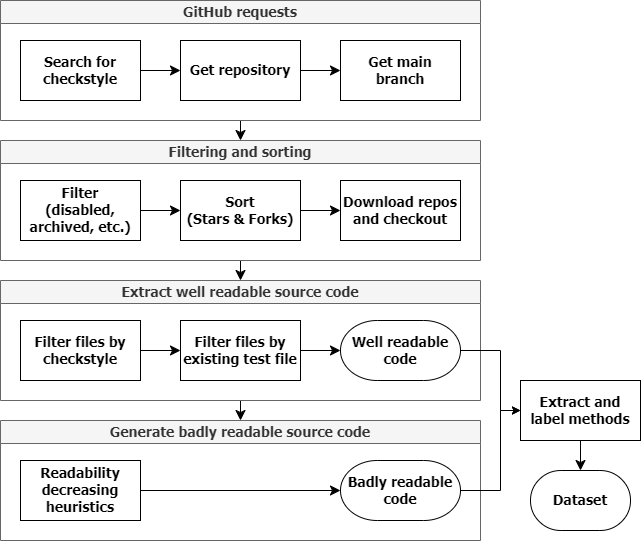
\includegraphics[width=\textwidth]{img/dataset_generation.png}
		\caption{The used dataset generation approach.}
		\label{fig:dataset_generation}
	\end{figure}
	
	The approach is divided into four parts. The first three steps are used to mine well readable java code. In a final step, we will modify the well readable code to achieve our second goal, namely poorly readable source code.
	
	We start by querying the GitHub REST API\curl{https://docs.github.com/en/rest}{2024-02-15} for repositories that use checkstyle (query string: "checkstyle filename:pom.xml"). The repository informations (including the URL) are stored together with the main branches.
	We remove all repositories that do not fulfill these criteria:
	\begin{itemize}
		\item The repository is not a fork of another repository
		\item The repository is not archived
		\item The repository is not disabled
		\item The repository language is Java
		\item The repository has at least 20 stars
		\item The repository has at least 20 forks
	\end{itemize}
	
	% TODO: Why miteinbauen oder eher nicht?
		
	The remaining ones are sorted by their star and fork count (equally weighted). The 100 best are cloned and their main branch is checked out.
	
	In a third step we run checkstyle (\curl{https://checkstyle.sourceforge.io/}{2024-02-15}) against the project own checkstyle configuration to get all java class files, that pass the own checkstyle test. From the java classes that passed this filter we extract all methods that have a comment of any kind at the beginning of the method. This results in 36077 code snippets which we assume to be well readable.
	
	The fourth and final step is to generate badly readable code from the well readable one. Therefore we use the proposed Readability Decreasing Heuristics (RDH, see section \ref{Readability Decreasing Heursitcs}). Afterwards we again extract all methods with a comment at the beginning of the method.
	Initially we planned to not require comments for the badly readable dataset part. However, it turns out that in this case all well-readable methods have a comment while most of the badly-readble do not have one. This lead to shortcut learning, whether a method has a comment or not instead of learning to distinguishing the methods by all other criteria as well.
	
\subsection{Readability Decreasing Heuristics} \label{Readability Decreasing Heursitcs}
	We already mentioned, that Readability Decreasing Heuristics (RDH) are used to generate badly readable code from well readable code. In this section we will explain how we achieved this and what is meant by RDH.
	The RDH are a set of code manipulation heuristics that are applied to Java files. One part is performed on the abstract syntax tree (AST) representation of the Java files using the spoon library (\curl{https://spoon.gforge.inria.fr/}{2024-15-02}) \cite{pawlak2016spoon}. Another part is performed when converting the AST back into Java files.
	From now on, we will use the abbreviation RDH or RDH tool when referring to the entire program. If a specific manipulation or a subset of all manipulations is meant, we will use [name] rdh instead.
	
	The RDH tool converts the Java code of each well readable Java class file into an AST. In the end the AST is parsed back to Java code using an pretty printer. If nothing else is done, this results in the "none" rdh. Note that the code produced by the tool in this way will be slightly different from the original input code, as the styling and formatting of the original code will be overwritten by the default formatting of the Java Pretty Printer of the spoon library.
	
	Various code changes can be made between the two steps and during printing (see Figure \ref{fig:rdh}).
	The renaming is done while the code is in its AST representation to ensure that the declarations and usages of variables, fields and methods are all renamed to the same new name. 
	The other transformations are performed when the AST is converted back to source code. This includes adding additional spaces, adding or removing newlines and changing the indentation of code in term of tabs.
	
	\begin{figure}[t]
		\centering
		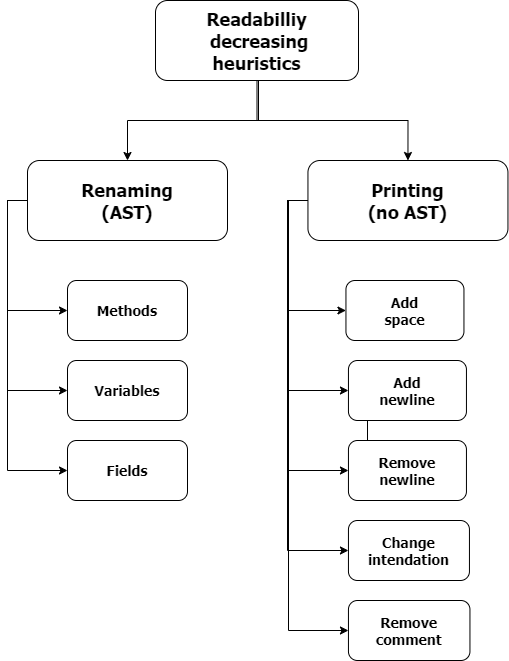
\includegraphics[width=0.5\textwidth]{img/rdh.png}
		\caption{The available Readability Decreasing Heuristics (RDH)}
		\label{fig:rdh}
	\end{figure}
	
	The individual methods are then extracted from the class files. As already mentioned, we need a method comment for all methods. We therefore use the RDH "remove-comment" after completing the method extraction.
	
	The RDH works with a configuration file in which one can specify a probability for each heuristic that can be applied. We have chosen the probabilities so that the generated code snippets are still realistic in the sense that they could also be written by humans. You can find the configuration file for the none rdh in Appendix \ref{app:TODO}.
	
	Some of the heuristics were not included in the final version of the new dataset. You can find them in table \ref{tab:not-included-rdhs} together with the reason why they were not included.
	
	\begin{table}[h]
		\centering
		\begin{tabular}{|c|c|}
			\hline
			\textbf{Heuristic} & \textbf{Reason} \\
			\hline
			\texttt{inlineMethod} & Makes methods to long \\
			\hline
			\texttt{add0} & Limited survey capacity \\
			\hline
			\texttt{insertBraces} & Limited survey capacity \\
			\hline
			\texttt{starImport} & No effect after comment extraction \\
			\hline
			\texttt{inlineField} & Limited survey capacity \\
			\hline
			\texttt{partiallyEvaluate} & Might increase readability \\
			\hline
		\end{tabular}
		\caption{Readability Decreasing Heuristics that are not included in the final version of the new dataset and why}
		\label{tab:not-included-rdhs}
	\end{table}
	
	We have also added Code2Vec~\cite{alon2019code2vec} to the tool. This makes it possible to rename methods not only to iterating or arbitrary strings or numbers, but also to other realistic method names. The idea was to use worse method names predicted by Code2Vec and rename the methods to these. However, due to time and resource constraints regarding the survey, we did not pursue this approach.	However, there is a corresponding mode supported by the tool. This can be used for further research.
	
\subsection{Survey} \label{Survey}
	We evaluated the data set generated and the new approach with a survey. To do this, we had to carefully select suitable code snippets from the dataset. An overview of the approach can be found in Figure \ref{fig:survey_pipeline}.
	
	\begin{figure}[t]
		\centering
		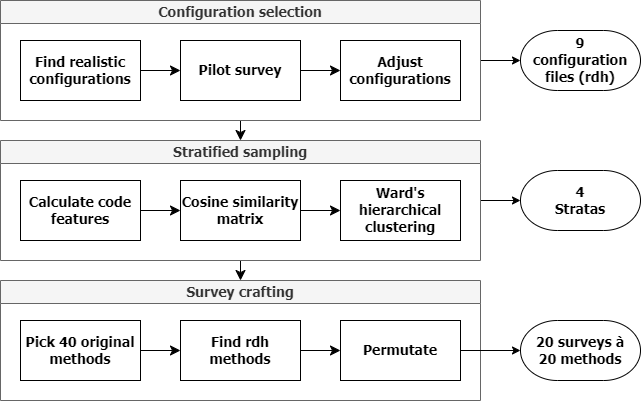
\includegraphics[width=\textwidth]{img/survey_pipeline.png}
		\caption{Steps performed to craft survey sheets from the dataset}
		\label{fig:survey_pipeline}
	\end{figure}
		
	The first step was to find realistic configurations for the readability reduction tool. After an initial data set with the heuristics was created, a pilot study was conducted. Subsequently, the heuristics that proved to be too strong were checked and, if necessary, adjusted to be weaker according to the results of the pilot survey. The result was 9 different rdhs, which can be found in table \ref{tab:rdh_configurations}. Together with the original methods this resulted in 10 different configurations.
	
	\begin{table}[h]
		\centering
		\begin{tabular}{|l|l|l|}
			\hline
			\textbf{Configuration} & \textbf{RDH probabilities} \\
			\hline
			none & - \\
			\hline
			comments\_remove & removeComment: 1.0 \\
			\hline
			newline\_instead\_of\_space & newLineInsteadOfSpace: 0.15 \\
			\hline
			newlines\_few & \begin{tabular}[t]{@{}l@{}}removeNewline: 0.3 \\ spaceInsteadOfNewline: 0.05\end{tabular} \\
			\hline
			newlines\_many & \begin{tabular}[t]{@{}l@{}}add1Newline: 0.15 \\ add2Newlines: 0.05\end{tabular} \\
			\hline
			rename & \begin{tabular}[t]{@{}l@{}}renameVariable: 0.3 \\ renameField: 0.3 \\ renameMethod: 0.3\end{tabular} \\
			\hline
			spaces\_many & \begin{tabular}[t]{@{}l@{}}Add1Space: 0.2 \\ Add2Spaces: 0.1 \\ spaceInsteadOfNewline: 0.05\end{tabular} \\
			\hline
			tabs & \begin{tabular}[t]{@{}l@{}}remove1IncTab: 0.2 \\ add1IncTab: 0.1 \\ remove1DecTab: 0.1 \\ add1DecTab: 0.1 \\ incTabInsteadOfDecTab: 0.05 \\ decTabInsteadOfIncTab: 0.05\end{tabular} \\
			\hline
			all7 & all probabilites/7\\
			\hline
		\end{tabular}
		\caption{Chosen configurations and their probabilities for the RDH tool}
		\label{tab:rdh_configurations}
	\end{table}
	
	The configurations are based on probabilities for different heuristics. A heuristic is applied with the specified probability to each occurrence of the object to which it is to be applied. For example, comment\_remove is applied with a probability of 10\% to each comment that occurs within the code snippet. The exact scope of changes for a method is therefore uncertain. It can even happen (especially with short methods such as getters and setters) that a method is not changed at all. For example, if a method only has a single comment and we use comment\_remove, it is very likely that the method will not be changed at all.
	
	In a second step, we applied a stratified sampling to distinguish between very simple methods such as getter and setter and more complex methods. In order to be able to compare the original methods with their modified variants, we only carried out the random sampling for the original methods and compared the rdh methods with these in a later step.
	
	Thus, we first had to calculate features for the original code snippets. This was done using \citeauthor{scalabrino2018comprehensive}s tool~\cite{scalabrino2018comprehensive}. Therefore, a 110-dimensional features vector was calculated for each original code snippet. Next we compute the cosine similarity metrix between all feature vectors using scikit\curl{https://scikit-learn.org/stable/modules/generated/sklearn.metrics.pairwise.cosine_similarity.html}{2024-02-20}. 
	Finally, using the fastcluster implementation \cite{mullner2013fastcluster} of Ward's hierarchical clustering we were able to cluster the methods into an arbitrary amount of clusters.	
		
	By comparing the merge distances in each step (see figure \ref{fig:survey_cluster_amount}), we found that a cluster size of 4 makes the most sense: the merge distance of 5 to 4 is small, so we should still perform this merge, but the merge distance of 4 to 3 is large, so it is better not to perform this merge. Also, 4 is the size with the last possibility for a small merge distance. We have manually assigned a name to each of the 4 cluster/strata, which can be seen in Table \ref{tab:survey_strata_labeles}.
	
	\begin{figure}[t]
		\centering
		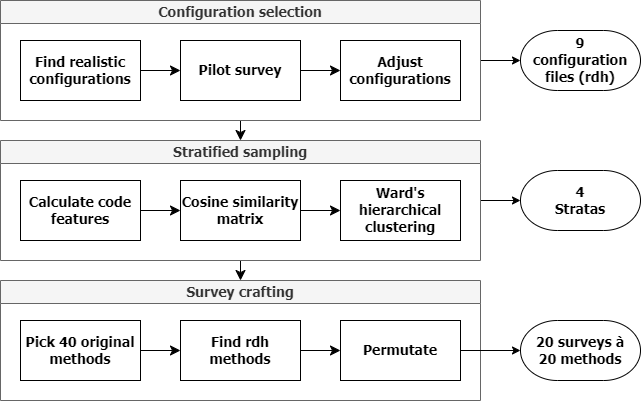
\includegraphics[width=\textwidth]{img/survey_pipeline.png}
		\caption{TODO: Replace. Merge difference and local derivative for amount of clusters/strata between 2 and 10} 
		\label{fig:survey_cluster_amount}
	\end{figure}
	
	\begin{table}[htbp]
		\centering
		\begin{tabular}{ll}
			\toprule
			\textbf{Stratum} & \textbf{Method Type} \\
			\midrule
			Stratum 0 & Simple methods \\
			Stratum 1 & Complex methods \\
			Stratum 2 & Magic number methods \\
			Stratum 3 & Medium complex methods \\
			\bottomrule
		\end{tabular}
		\caption{Computed stratas and manually assigned name based on the methods within}
		\label{tab:survey_strata_labeles}
	\end{table}
		
	In the third step, we crafted the surveys from the layers. We decided to provide all 10 previously mentioned configurations for each original method, as we want to compare the original methods with their rdh variants. Since we have a survey capacity of 400 code snippets, we need to select 40 original code snippets (and then add all their rdh).	
	
	We chose to sample randomly from within the stratas. However, we distributed the 40 snippets among the stratas as can be seen in table \ref{tab:sampled_methods}.
	
	We opted for a random sample within the strata. However, we distributed the 40 snippets across the strata as shown in Table~\ref{tab:sampled_methods}.
	
	\begin{table}[htbp]
		\centering
		\begin{tabular}{lccc}
			\toprule
			\textbf{Stratum} & \textbf{Percentage} & \textbf{Count} \\
			\midrule
			Stratum 0 & 10\% & 4 \\
			Stratum 1 & 40\% & 16 \\
			Stratum 2 & 10\% & 4 \\
			Stratum 3 & 40\% & 16 \\
			\midrule
			\textbf{Total} & \textbf{100\%} & \textbf{40} \\
			\bottomrule
		\end{tabular}
		\caption{Strata distribution of sampled methods}
		\label{tab:sampled_methods}
	\end{table}
	
	This decision was made due to the relatively high frequency of methods that do not differ from their original methods (see Figure \ref{fig:sampling_not_different_overall}). Another reason for this decision is that particularly simple methods are rather uninteresting for the classification of readability, as they are often generated (e.g. by IDEs) and usually follow a straightforward pattern.
	
	\begin{figure}[t]
		\centering
		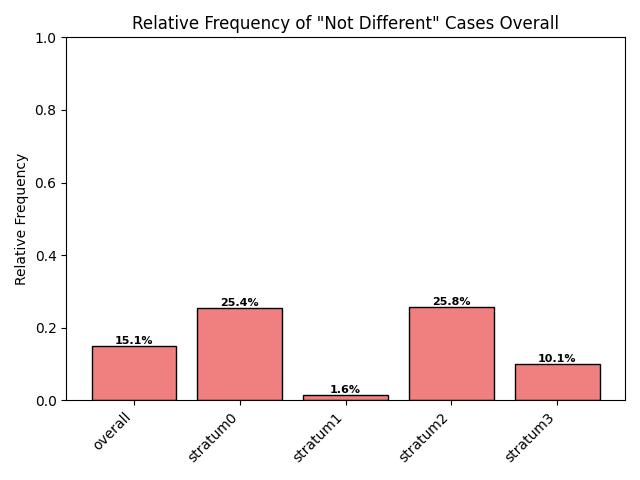
\includegraphics[width=\textwidth]{img/sampling_not_different_overall.png}
		\caption{Relative frequency of the case that a rdh-method is not different from it's original method.} 
		\label{fig:sampling_not_different_overall}
	\end{figure}
		
	After selecting the 40 original methods, we next selected all 9*40 rdh variants that belong to the original methods. This was mostly done automatically based on the names of the original methods and the names of the rdh variant methods. However, if the method was renamed at an earlier stage due to the method renaming heuristic, the new method did no longer match the original method, so we had to match them manually.
		
	Once we had collected all 400 methods, we had to distribute them across the 20 survey forms, each with 20 methods. In order not to manipulate the raters, we decided that a variant of each method could only appear once in each survey sheet. For example, if the original method is in questionnaire 1, the comment\_remove variant (or another variant of the same method) must not be included in the same questionnaire.
		
	For this purpose, we created four permutation matrices with 10 snippets each. The number 10 was chosen because it is possible to distribute 10 snippets, each with 10 variants, to at least 10 survey arcs without violating our condition. By combining two 10-permutation matrices, we were able to create 10 survey arcs with 20 code snippets each. An implication of this approach is that each survey sheet contains each variant exactly twice. By doing this twice, we obtain the desired distribution of 20 survey questionnaires with 20 methods each. Our condition also applies: There is only one variant of the same method in each questionnaire.
		
	Finally, the methods for each survey questionnaire were randomly shuffled within each survey questionnaire. This was done to minimize the impact of the position of a snippet/variant within a survey on the rating.			
	
\subsection{Readability Classification Model} \label{Readability Classification Model}
	We will investigate whether it is possible to score a higher accuracy as current models in classifying code readability for Java using Deep Learning. Therefore, we will train the model from \citeauthor{mi2022towards}~\cite{mi2022towards} with more data. We will consider augmenting the model with a method name classifier and incorporating semantic encoding for tabs and spaces. The training data will be generated in a novel way for classification of readability, inspired by \citeauthor{loriot2022styler}~\cite{loriot2022styler}. The method name classifier is similar to Code2Vec~\cite{alon2019code2vec}. The combination of all components is novel to the best of our knowledge. You can find a visualization of the planned modifications of \citeauthor{mi2022towards}'s model in figure~\ref{fig:model_pipeline}. We will focus on generating training data, as the approach will be usable for further research in the field of source code readability.
	
	\begin{figure}[t]
		\centering
		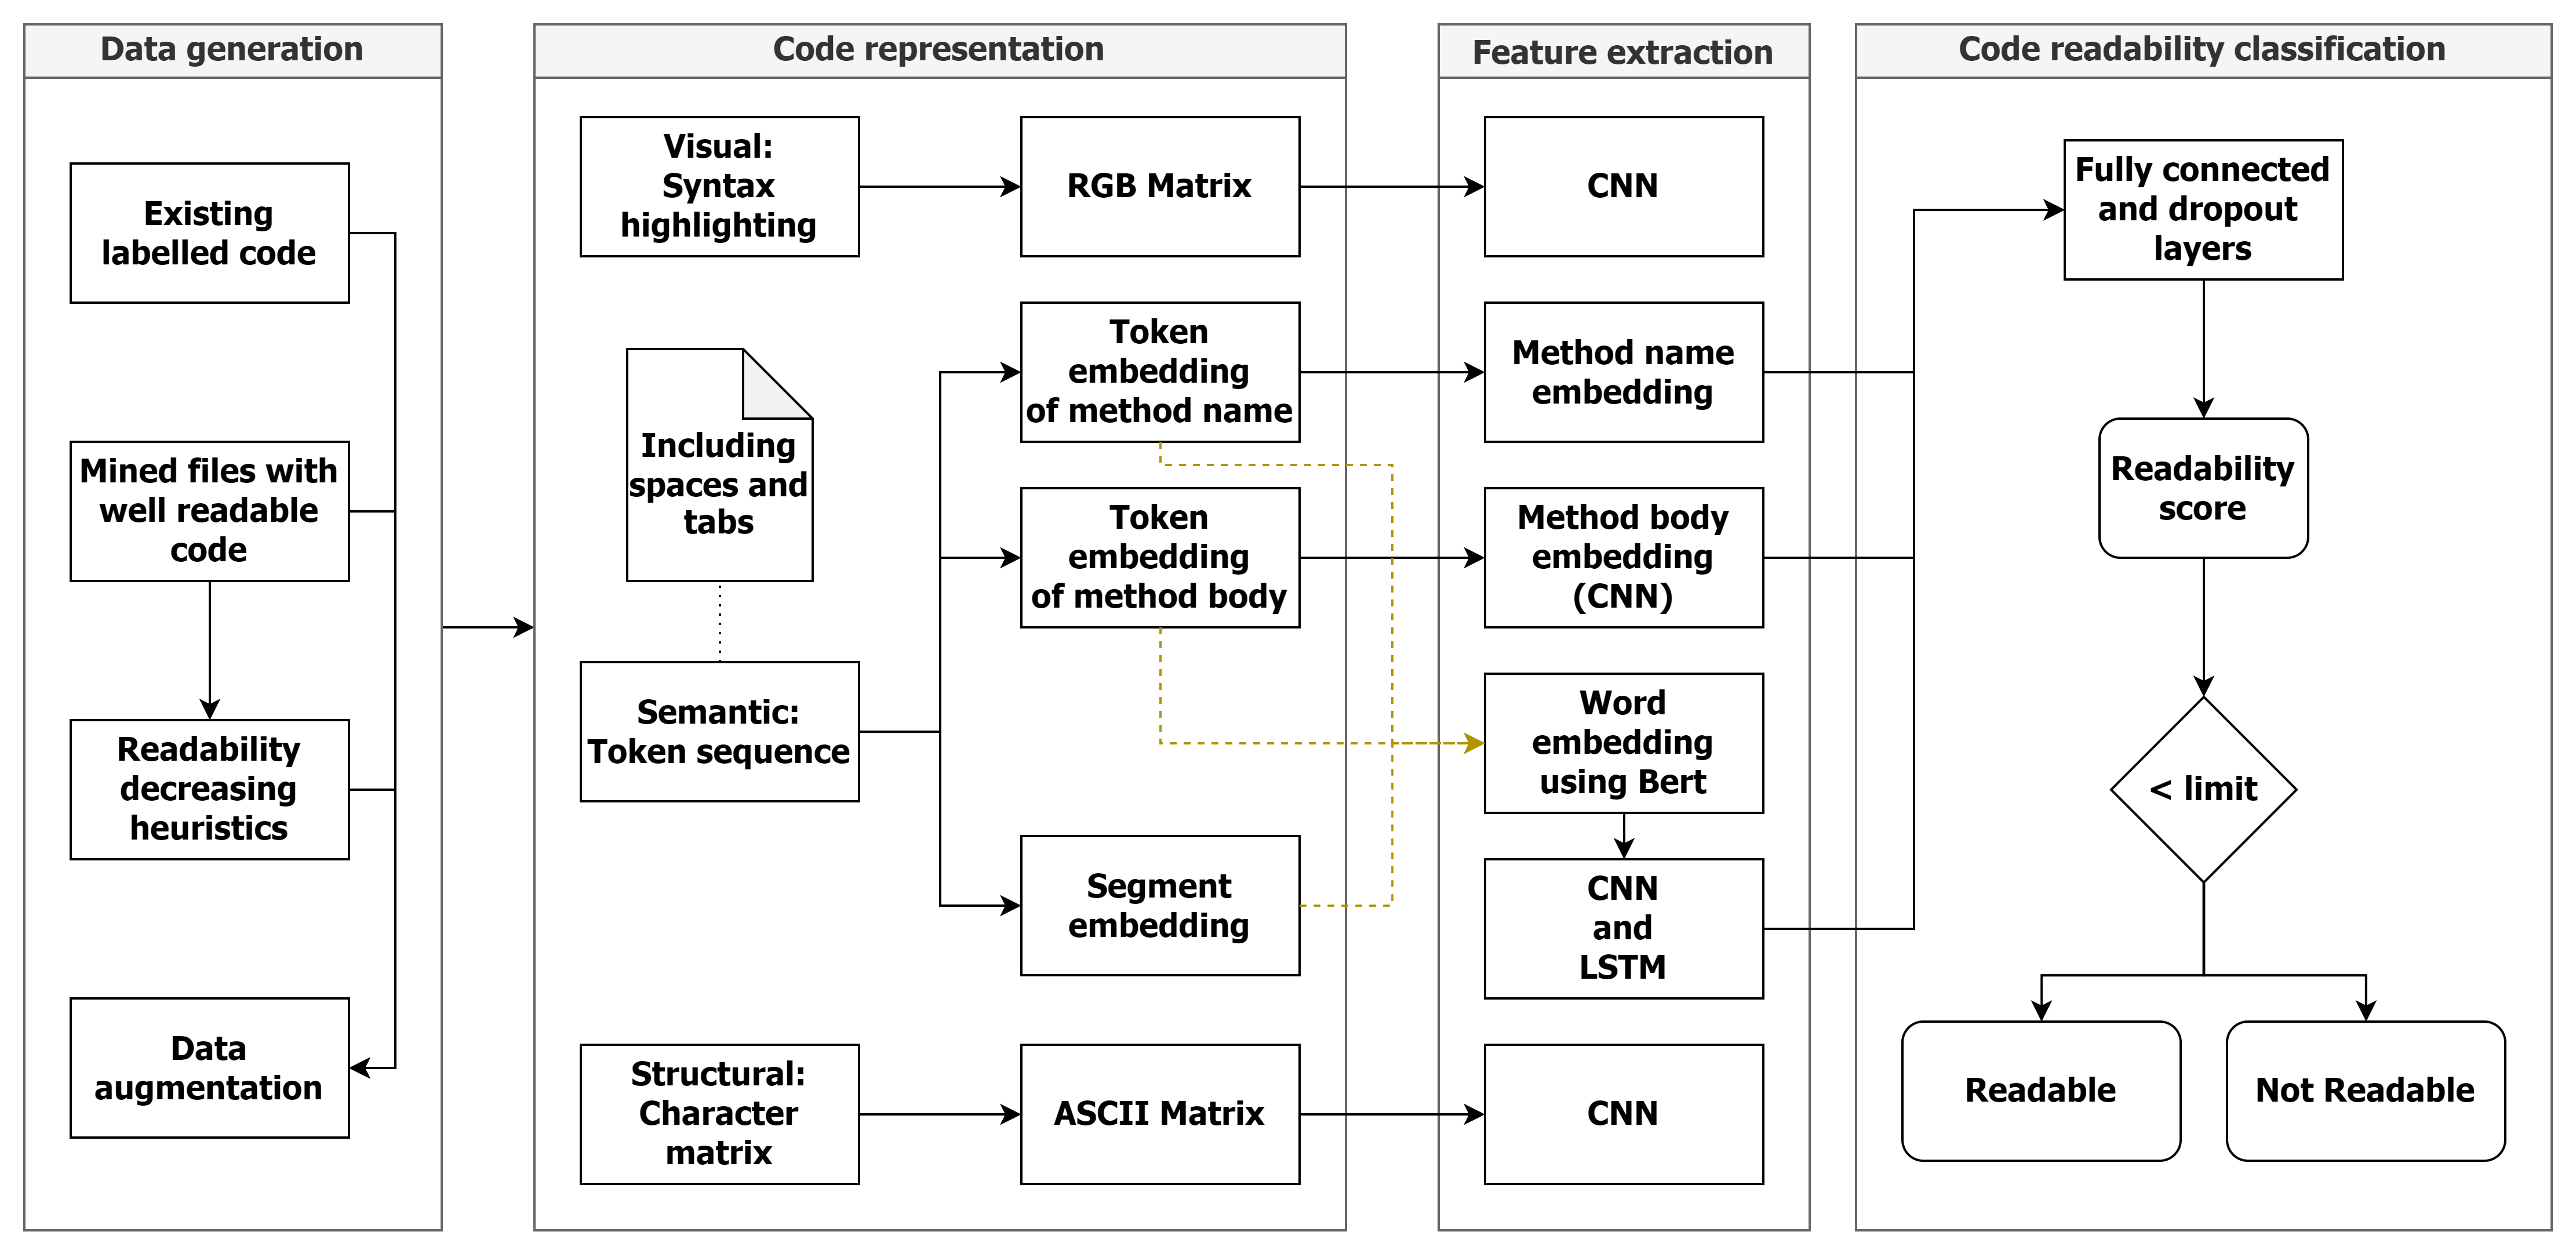
\includegraphics[width=\textwidth]{img/model_pipeline_old.png}
		\caption{Overview of the planned approach.}
		\label{fig:model_pipeline}
	\end{figure}
	
	% TODO: Inline this in research questions?
	% \subsection{Data generation} \label{Data generation}
	Deep Learning based models perform better the more training data they get~\cite{hestness2017deep}. Therefore, one approach in order to further improve existing models is to gather more training data.
	This requires, as it was done previously, a lot of effort and persons willing to rate code based on their readability. We present another approach for gathering training data.
	
	In a first step, GitHub repositories with known high code quality are downloaded and labeled as highly readable. We select repositories using a similar approach as \citeauthor{allamanis2016convolutional}~\cite{allamanis2016convolutional} and then assume that they contain only well readable code.
	In a second step, the code is manipulated so that it is subsequently less readable. This approach is similar to the approach of \citeauthor{loriot2022styler}~\cite{loriot2022styler}. After both steps, we have a new, automatically generated training dataset for source code readability classification.
		
	% Readabililty Decreasing Heuristics
	This brings up the question, how to manipulate code so that it is less readable afterwards. We therefore introduce a tool called Readability Decreasing Heuristics. As the name suggests this is a collection of heuristics that, when applied to source code, lower the readability of it. For example such a heuristic is to replace spaces with newlines. Another example is to increase the indentation of a code block by a tab or multiple spaces. Moreover, with most changes it is also possible to do exactly the opposite (replacing newlines with spaces, decreasing indentation), which in most cases also decreases the readability of source code.
	
	Code snippets in Java are syntactically the same, before and after applying Readability Decreasing Heuristics. Complexity did not change either. However, if various modifications are applied many times, those changes are capable of lowering the readability of source code, as the comparison of listing~\ref{lst:cassandra-src-java-org-apache-cassandra-utils} and listing~\ref{lst:cassandra-src-java-org-apache-cassandra-utils-modified} suggests.
	
	Note that we assume two things for the data generation approach:
	\begin{enumerate}[label={Assumption \arabic*},ref={\arabic*},leftmargin=*]
		\item \label{well-readable-assumption} \textbf{(well-readable-assumption)} The selected repositories contain only well-readable code.
		\item \label{poorly-readable-assumption} \textbf{(poorly-readable-assumption)} After applying Readability Decreasing Heuristics, the code is poorly readable.
	\end{enumerate}
	
	% Model modifications/Further improvements
	\label{model-modifications}
	In recent years it was shown that Deep Learning models can be further improved by modifying the structure of the architecture or by introducing new components, parts or layers to existing architectures. 
	We suggest two improvements for the model of \citeauthor{mi2022towards}~\cite{mi2022towards}. Firstly, we want to embed spaces and tabs as semantic tokens. Secondly, adding a method name fitting classifier as a component of the overall model could be an improvement.
	% Surpassing
	\label{suggestions}If there is time left, we will try to surpass the performance of recent source code readability classifiers with those improvements to data generation and the model.
	%, such as the model proposed by \citeauthor{mi2022towards}~\cite{mi2022towards}.
	
	% We suggest two improvements for the model of \citeauthor{mi2022towards}~\cite{mi2022towards}:
	%\begin{enumerate}
	%	\item \label{embedding-spaces-component} \textbf{(embedding-spaces-component)} Embedding spaces and tabs as semantic tokens.
	%	\item \label{name-classifier-component} \textbf{(name-classifier-component)} Adding a method name fitting classifier as a component of % the overall model.
	%\end{enumerate}
	
	We will evaluate our suggestions with two methods. Firstly, we conclude a user study. Secondly, we compare code readability models with each other.
	
	\pagebreak
	
\subsection{Code base} \label{Code base}
	Our code is available on GitHub. TODO: Refs
	
	You can find an overview over all programs used to create the merged dataset, the new dataset the model and all our evaluation results in Figure \ref{fig:scripts_pipline}.
	
	\begin{figure}[t]
		\centering
		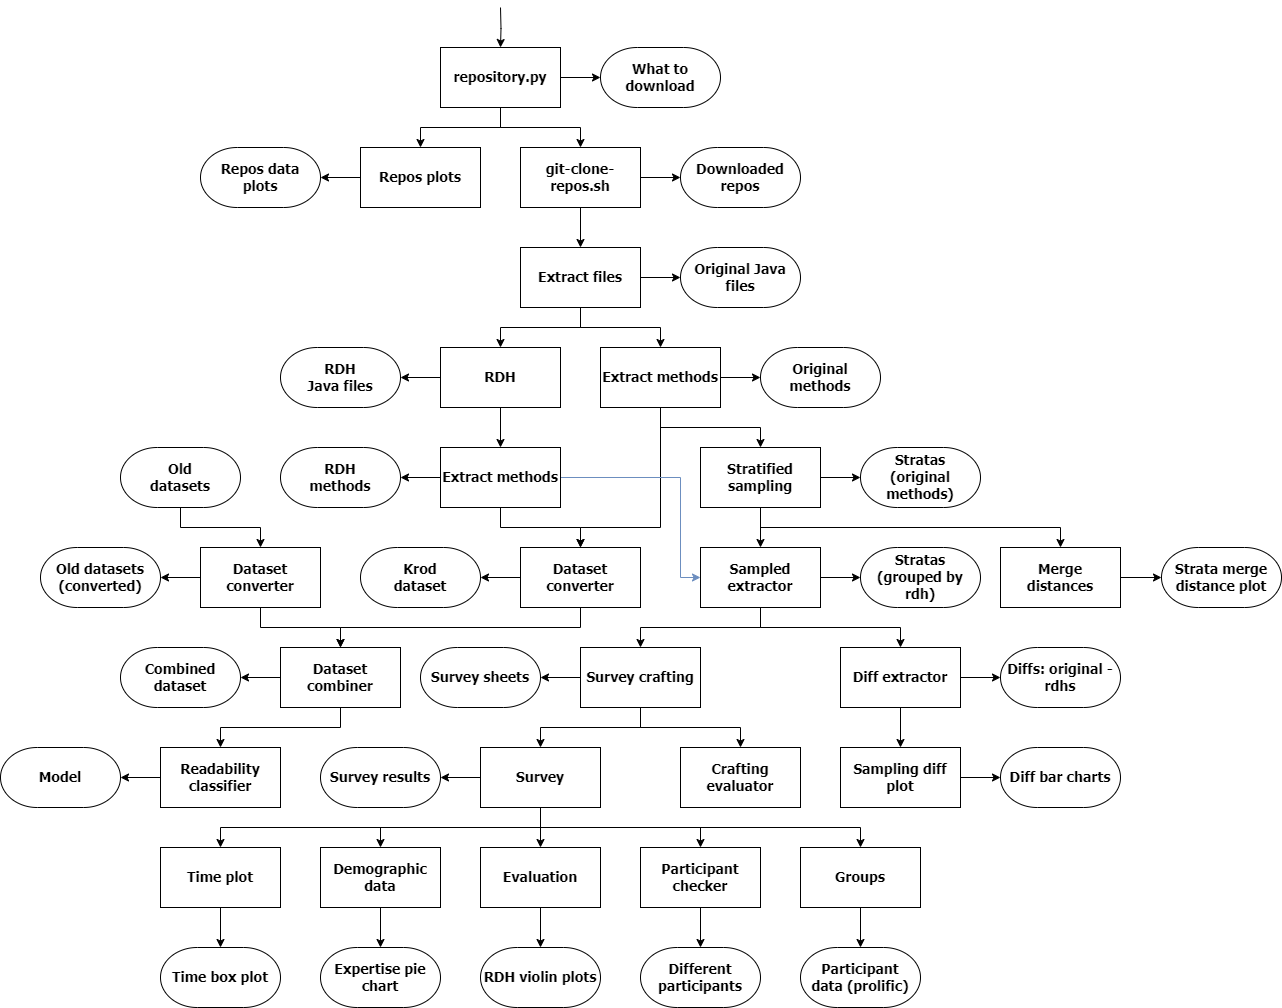
\includegraphics[width=\textwidth]{img/scripts_pipeline.png}
		\caption{Overview over the used scripts and their output}
		\label{fig:scripts_pipline}
	\end{figure}
	
	While re implementing the original model we came across the following possible issue of the model:
	The token length for the bert encoding (bert-base-cased) used within the model is set to 100. What is a token in a piece of code? Besides special tokens to mark the beginning [CLS] and end [SEP] of the input, each word is represented by a token. However, also each special character (such as /(){},;= and many more) is represented by a own token. Java identifiers are split using the camel case convention. Long words are split again into multiple tokens.
	
	Consider the method from Listing \ref{lst:cassandra-src-java-org-apache-cassandra-utils}. With a token limit of 100, the last encoded token is the last closing brace in line 9. Everything from line 10 onward is not encoded anymore, which means, that the information is lost for the semantic encoder. To put it in other words: The model of \citeauthor{mi2022towards} considers only the first few lines of code snippets in it's semantic component.
	
	The visual and structural have similar limitations, however, they are less conservative. The structural encoder encodes the first 50 lines of each code snippet and the visual encoder encodes the first 43 lines. While the restrictions for both of those encoders seem to be long enough to capture most of the code snippets fully, the semantic encoder seems to be too limited to capture most of the code snippets fully. One reason for this could be, that the first part of a method is of higher semantic importance.
	
	While we want to remark these limitations, we will stick with them to allow later a fair comparison of the datasets against the model of of \citeauthor{mi2022towards} trained on the combined dataset.	
	
\subsection{User study}\label{user-study}
	% We will conclude a user study to evaluate the newly generated data for readability classifier models.
	The goal of the user study is to answer the following key questions:
	
	\begin{enumerate}
		\item Does the well-readable-assumption (assumption \ref{well-readable-assumption}) hold?
		\item Does the poorly-readable-assumption (assumption \ref{poorly-readable-assumption}) hold?
	\end{enumerate}
	
	We will achieve this by showing programmers code snippets that were generated with the presented approach. Therefore, human annotators give each code snippet a rating of its readability. The annotators are selected by prolific\curl{https://www.prolific.com/}{2023-09-30}. Particular attention is paid to a high proportion of people from industry. The readability rating is based on a five-point Likert scale~\cite{likert1932technique} ranging from one (i.e., very unreadable) to five (i.e., very readable). We apply the same rating as done previously~\cite{buse2009learning, dorn2012general, scalabrino2018comprehensive}, but, other than before, we will not use the rating for labeling the training data. Instead, we will only use the ratings to validate a few randomly selected code snippets out of many that are automatically labeled.
		
	\subsubsection{Comparing models}\label{compare-models}
	Besides the user study we will evaluate our suggestions by comparing machine learning models against each other.
	The comparisons are based on common metrics such as accuracy, F1-score and MCC~\cite{chicco2020advantages}. One can distinguish further between the following variants of comparing models:
	
	In one variant we compare models that have the same architecture (same layers, same weight initialization, same components, etc.) while they differ in the data they are trained on. For example, we can train a model with the old and new datasets, separately and combined. If done for multiple model architectures we can evaluate how the differences in training data influence the model performance. 
	
	Another variant would be to compare models with different architecture but the same training data. In this way, we can evaluate newly introduced components by measuring and comparing the performance of such models.

	A third comparison variant is created by combining the first two. Both of them lead to many options in what to compare, especially if only small changes to training data or model architecture are done. To find out, if our suggestions lead to a better model overall, we will compare our newly created model with all changes at once to the state-of-the-art model of \citeauthor{mi2022towards}~\cite{mi2022towards}.
	
	\subsubsection{Research questions}\label{research-questions}
	We come up with the following research questions:
	
%	\begin{resq}What is the quality of our new approach for data generation?\end{resq} \label{RQ1}
%	Until now, the data for readability classification was generated manually. Therefore, human annotators ranked code snippets by their readability level based on a five-point Likert scale~\cite{likert1932technique} ranging from one (i.e., very unreadable) to five (i.e., very readable)~\cite{buse2009learning, dorn2012general, scalabrino2018comprehensive}. Our new data will be generated in an automatic approach, where no manual labeling of code is necessary. We want to compare the quality of this data to the data used for previous models.
	
	\begin{resq} \textbf{(select-well)} Can automatically selected code be assumed to be well readable?\end{resq} \label{select-well}
	In our new approach for generating training data, we assume that the code from repositories is readable under certain conditions (assumption~\ref{well-readable-assumption}). We want to check whether that holds. To answer this question we will use the results of the user study (section~\ref{user-study}).
	
	\begin{resq} \textbf{(generate-poor)} Can poorly readable code be generated from well readable code?\end{resq} \label{generate-poor}
	It is not sufficient to have only well readable code for training a classifier. We also need poorly readable code. Therefore, we will try to generate such code from the well readable code. We will investigate whether this is possible in principle, and we will propose an automated approach for archiving this: Readability Decreasing Heuristics.
	
	As the name already suggests, the applied transformations on the source code are only heuristics. To answer, whether the generated code is badly readable (assumption~\ref{poorly-readable-assumption}) we will utilize the results of the user study (section~\ref{user-study}).
	
	\begin{resq} \textbf{(best-heuristics)} Which heuristics are best to generate poorly readable code from well readable code?\end{resq} \label{best-heuristic}
	We want to compare the modifications of the proposed heuristics for generating poorly readable code to each other. Therefore we will train the same classifier model with badly readable code generated by different Readability Decreasing Heuristics. We will then evaluate the model variations against each other (section~\ref{compare-models}) to answer the research question.
	
	\begin{resq} \textbf{(new-data)} To what extent can the new data improve existing readability models?\end{resq} \label{new-data}
	It was shown that Deep Learning models get better the more training data is available~\cite{hestness2017deep}. This holds under the assumption that the quality of the data is the same or at least similar. We want to check if the quality of our new data is sufficient for improving the Deep Learning based readability classifier of \citeauthor{mi2022towards}~\cite{mi2022towards}. Therefore we will train their proposed model with and without the new data and then evaluate the models against each other (section~\ref{compare-models}).
	
	% Next RQ on new page
	\pagebreak
	
%	\begin{resq} \textbf{(model-modifications)} Optional: How can existing Deep Learning approaches be further improved?\end{resq} \label{model-modifications}
%	In recent years it was shown that Deep Learning models can be further improved by modifying the structure of the architecture or by introducing new components, parts or layers to existing architectures. We suggest two improvements for the model of \citeauthor{mi2022towards}~\cite{mi2022towards}: Embedding spaces and tabs as semantic tokens and adding a method name fitting component. We will evaluate the proposed improvements as described earlier~\ref{suggestions}.
	
	\begin{resq} \textbf{(embedding-spaces)} Optional: To what extend does the embedding of spaces and tabs in semantic code representations improve readability classification?\end{resq} \label{embedding-spaces}
	The state-of-the-art model of \citeauthor{mi2022towards}~\cite{mi2022towards} does consider spaces and tabs only in its visual component. We want to investigate if it can improve the quality of a Deep Learning based model if spaces and tabs are encoded as semantic tokens. We also want to investigate if this makes the visual component superfluous. We will evaluate the proposed improvement as described earlier (section~\ref{compare-models}).
	
	\begin{resq} \textbf{(name-classifier)} Optional: To what extend does the usage of a method name classifier improve readability classification?\end{resq} \label{name-classifier}
	Correct naming of identifiers is crucial for ensuring readability of software programs. It is of outstanding importance for readability of code that the name of methods fit the method bodies~\cite{liu2019learning}. We want to introduce a new component to the model of \citeauthor{mi2022towards}~\cite{mi2022towards} that is built similar to Code2Vec~\cite{alon2019code2vec}. We want to investigate if the newly introduced component improves the quality of the resulting model. We will evaluate the proposed improvement as previously described (section~\ref{compare-models}).
	
\section{Evaluation} \label{Evaluation}
In this section we will present our evaluation results.

\subsection{Survey Results} \label{Survey Results}
	The results from our survey are separated into two parts: The results from the pilot survey used to improve the main survey pre start and the main survey results used to answer our research questions.

\subsubsection{Pilot survey} \label{Pilot Survey}
	The pilot survey was used to adjust the rdh-probability settings and the survey itself before start.
	
	The pilot survey gave an insight into how much time one would need to rate 20 code snippets regarding it's readability. You can find an overview over the times needed in Figure \ref{fig:pilot_survey_time_box.png}. Based on this we estimated the time requirement for our survey with 10 minutes.
	
	\begin{figure}[t]
		\centering
		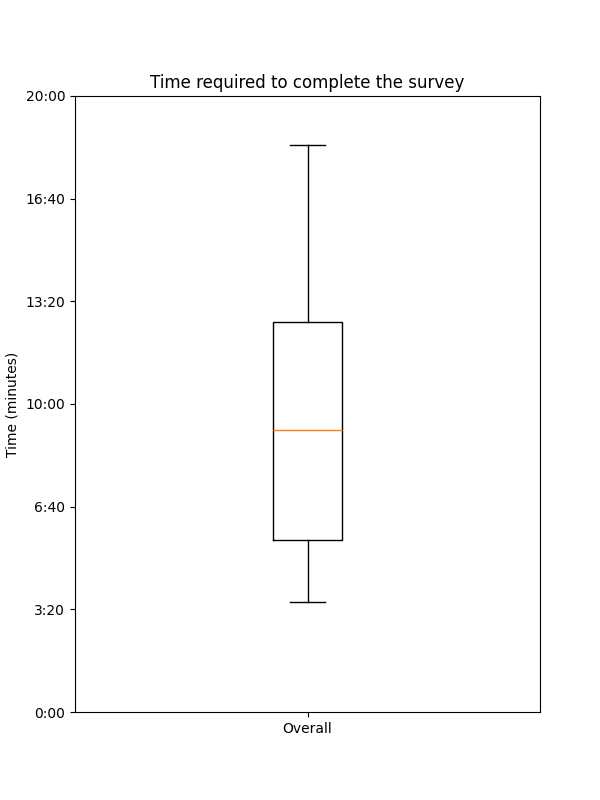
\includegraphics[width=\textwidth]{img/survey_time_box.png}
		\caption{TODO: Replace with actual one.}
		\label{fig:pilot_survey_time_box.png}
	\end{figure}
	
	Most of the problems that came up where due to the survey tool (for example: "I also thought that I should use the drop-down menu on the upper left."). You can find all feedback in appendix TODO.
	
	%	It is sometimes necessary to swipe horizontally to see all of the code, which is a bit inconvenient.
	%	After finishing the task, at least message should be shown.
	%	First I needed to figure out how this tool works and that the rating is done with the stars below. I thought I should write my rating as a comment in the comment field below. After number 20 I didn't know whether I could close the survey or not.
	%	I also thought that I should use the drop-down menu on the upper left.
	%	Mobile is not easy to use because of the scrolling needed to complete the survey
	%	I didn't understand what the button at the top left meant, where you could select the programming language. There were too many fonts to choose. I also wasn't sure whether to write a comment or not. It wasn't described at the beginning.
	%	I suggest to make the task description accessible during the rating
	%	Submit vote after the last question could contain that one can close the survey now.
	%	Maybe the option to leave the survey, when clicking to submit.
	%	I would leave out the buttons described above. I was missing a scrollbar at the bottom of the code-window. A conclusion page with a message like "Thank you for your participation", "You're Done!" or other further information was missing, too.
	%	There werde drop downs for the programming language, but choosing another language did not change anything.
	%	9:53
	%	Das müsste alles Feedback zum Tool sein, ich schau mal, ob ich das auf die schnelle noch etwas zusammenfassen kann :slightly_smiling_face:
	%	9:57
	%	Zusammengefasst:
	%	Feature Request: "You're done! Thank you for your participation!" - message at the end
	%	Feature Request: Hide comment fields
	%	Feature Request: Predefine code parser (per survey/snippet) and hide selection during survey for participants
	%	Feature Request: Possibility to show a hint or the task description again during the survey
	
	Additionally some manual evaluation of the different rdhs, especially for stratum 1 suggested a few things:
	
	First of all, original methods where rated comparably well, which suggests the well-readable-assumption to hold.
	
	Secondly, the rdh tool did always fully declare each imported method or class with its fully specified classifier. For example, instead of 
	"InputStream", "java.io.InputStream" was declared. This gave the raters the feeling, that the code was actually not written by a human and drastically decreased it's readability. Afterwards, we adjusted the rdh-tool to not print the fully qualified name anymore. This has however the drawback, that it can not be guaranteed anymore that the generated code compiles and does the same as it's original. However, this property was lost anywhere upon extracting the individual methods from the class files.
	
	Third, some rdhs where configured to strong so that some methods were again not presumed to be written by a human anymore. These rdhs were adjusted and their probabilities were decreased accordingly (for example newlines\_few). For all results see Table \ref{tab:pilot_survey_results}.
	
	%	\begin{table}[htbp]
		%		\centering
		%		\begin{tabular}{llp{6cm}c}
			%			\toprule
			%			\textbf{Stratum} & \textbf{RDH} & \textbf{File} & \textbf{Score} \\
			%			\midrule
			%			stratum\_0 & spaces\_few & \seqsplit{hadoop\_FilePosition.java\_bufferFullyRead.java} & 3 \\
			%			stratum\_0 & tabs\_few & \seqsplit{hadoop\_DataNodeFaultInjector.java\_delayWriteToDisk.java} & 4,3 \\
			%			stratum\_1 & all & \seqsplit{hudi\_HoodieMultiTableStreamer.java\_populateTableExecutionContextList.java} & 1,2 \\
			%			stratum\_1 & all\_weak & \seqsplit{flink\_SSLUtils.java\_createInternalNettySSLContext.java} & 1,3 \\
			%			stratum\_1 & newlines\_few & \seqsplit{hudi\_Pipelines.java\_hoodieStreamWrite.java} & 1,7 \\
			%			stratum\_1 & spaces\_many & \seqsplit{hadoop\_ActiveAuditManagerS3A.java\_createExecutionInterceptors.java} & 2,1 \\
			%			stratum\_1 & tabs\_few & \seqsplit{hbase\_ZKMainServer.java\_main.java} & 2,2 \\
			%			stratum\_1 & tabs\_many & \seqsplit{flink\_HiveParserSemanticAnalyzer.java\_findCTEFromName.java} & 2,2 \\
			%			stratum\_1 & misc & \seqsplit{hbase\_Encryption.java\_decryptWithSubjectKey.java} & 2,4 \\
			%			stratum\_1 & spaces\_few & \seqsplit{hbase\_HBaseZKTestingUtility.java\_startMiniZKCluster.java} & 2,6 \\
			%			stratum\_1 & newlines\_many & \seqsplit{pulsar\_LoadSimulationController.java\_writeProducerOptions.java} & 2,9 \\
			%			stratum\_1 & all\_weak\_3 & \seqsplit{hadoop\_SingleFilePerBlockCache.java\_getIntList.java} & 3 \\
			%			stratum\_1 & comments\_remove & \seqsplit{flink\_MemorySegment.java\_get.java} & 3,1 \\
			%			stratum\_1 & methods & \seqsplit{flink\_HiveParserSemanticAnalyzer.java\_processPTFSource.java} & 3,7 \\
			%			stratum\_2 & newlines\_few & \seqsplit{zxing\_ModulusPoly.java\_isZero.java} & 2,4 \\
			%			stratum\_2 & methods & \seqsplit{hibernate-validator\_PESELValidator.java\_year.java} & 3,7 \\
			%			stratum\_2 & tabs\_few & \seqsplit{framework\_WindowMoveListener.java\_getTicketNumber.java} & 3,8 \\
			%			stratum\_3 & tabs\_many & \seqsplit{hadoop\_S3AInputPolicy.java\_getPolicy.java} & 1,7 \\
			%			stratum\_3 & newlines\_many & \seqsplit{hadoop\_CompressionCodec.java\_createInputStreamWithCodecPool.java} & 3,3 \\
			%			stratum\_3 & methods & \seqsplit{hbase\_PreviousBlockCompressionRatePredicator.java\_updateLatestBlockSizes.java} & 4,6 \\
			%			\bottomrule
			%		\end{tabular}
		%		\caption{Data with Highlighted Row}
		%		\label{tab:pilot_survey_results}
		%	\end{table}
	
	\begin{table}[htbp]
		\centering
		\begin{tabular}{llp{6cm}c}
			\toprule
			\textbf{Stratum} & \textbf{Feature} & \textbf{File} & \textbf{Score} \\
			\midrule
			stratum\_3 & methods & \seqsplit{hbase\_PreviousBlockCompressionRatePredicator.java\_updateLatestBlockSizes.java} & 4,6 \\
			stratum\_0 & tabs\_few & \seqsplit{hadoop\_DataNodeFaultInjector.java\_delayWriteToDisk.java} & 4,3 \\
			stratum\_2 & tabs\_few & \seqsplit{framework\_WindowMoveListener.java\_getTicketNumber.java} & 3,8 \\
			stratum\_1 & methods & \seqsplit{flink\_HiveParserSemanticAnalyzer.java\_processPTFSource.java} & 3,7 \\
			stratum\_2 & methods & \seqsplit{hibernate-validator\_PESELValidator.java\_year.java} & 3,7 \\
			stratum\_3 & newlines\_many & \seqsplit{hadoop\_CompressionCodec.java\_createInputStreamWithCodecPool.java} & 3,3 \\
			stratum\_1 & comments\_remove & \seqsplit{flink\_MemorySegment.java\_get.java} & 3,1 \\
			stratum\_0 & spaces\_few & \seqsplit{hadoop\_FilePosition.java\_bufferFullyRead.java} & 3 \\
			stratum\_1 & all\_weak\_3 & \seqsplit{hadoop\_SingleFilePerBlockCache.java\_getIntList.java} & 3 \\
			stratum\_1 & newlines\_many & \seqsplit{pulsar\_LoadSimulationController.java\_writeProducerOptions.java} & 2,9 \\
			stratum\_1 & spaces\_few & \seqsplit{hbase\_HBaseZKTestingUtility.java\_startMiniZKCluster.java} & 2,6 \\
			stratum\_1 & misc & \seqsplit{hbase\_Encryption.java\_decryptWithSubjectKey.java} & 2,4 \\
			stratum\_2 & newlines\_few & \seqsplit{zxing\_ModulusPoly.java\_isZero.java} & 2,4 \\
			stratum\_1 & tabs\_few & \seqsplit{hbase\_ZKMainServer.java\_main.java} & 2,2 \\
			stratum\_1 & tabs\_many & \seqsplit{flink\_HiveParserSemanticAnalyzer.java\_findCTEFromName.java} & 2,2 \\
			stratum\_1 & spaces\_many & \seqsplit{hadoop\_ActiveAuditManagerS3A.java\_createExecutionInterceptors.java} & 2,1 \\
			stratum\_1 & newlines\_few & \seqsplit{hudi\_Pipelines.java\_hoodieStreamWrite.java} & 1,7 \\
			stratum\_3 & tabs\_many & \seqsplit{hadoop\_S3AInputPolicy.java\_getPolicy.java} & 1,7 \\
			stratum\_1 & all\_weak & \seqsplit{flink\_SSLUtils.java\_createInternalNettySSLContext.java} & 1,3 \\
			stratum\_1 & all & \seqsplit{hudi\_HoodieMultiTableStreamer.java\_populateTableExecutionContextList.java} & 1,2 \\
			\bottomrule
		\end{tabular}
		\caption{Overview over the pilot survey results.}
		\label{tab:pilot_survey_results}
	\end{table}
	
	After the feedback regarding the survey tool was implemented, the actual study was conducted.

\subsubsection{Prolific Study Results} \label{Prolific Study Results}
	In this section we will summarize the results of the main study conducted via prolific.
	
	You can find an overview over the time required by the participants in the Figures \ref{fig:survey_time_box} and \ref{fig:survey_time_histogramm}. Additionally you can find the amount of participants that required less than 3 minutes for one survey sheet in Figure \ref{fig:survey_time_less_than_180}. The results of those participants might be a thread to validity to which we will come back later.
	
	\begin{figure}[t]
		\centering
		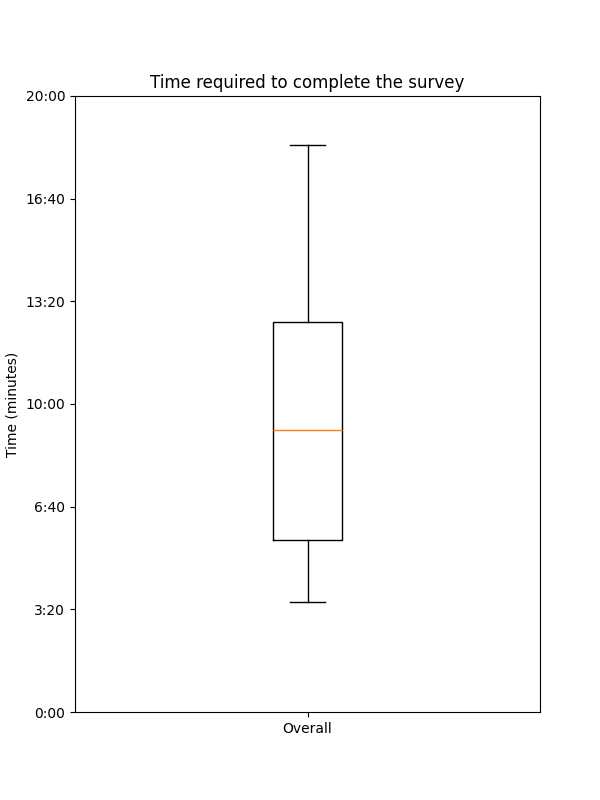
\includegraphics[width=\textwidth]{img/survey_time_box.png}
		\caption{Time required by the participants to complete the survey}
		\label{fig:survey_time_box}
	\end{figure}
	
	\begin{figure}[t]
		\centering
		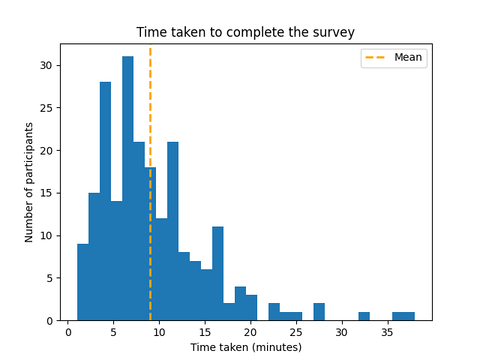
\includegraphics[width=\textwidth]{img/survey_time_histogramm.png}
		\caption{Time required by the participants to complete the survey}
		\label{fig:survey_time_histogramm}
	\end{figure}
	
	\begin{figure}[t]
		\centering
		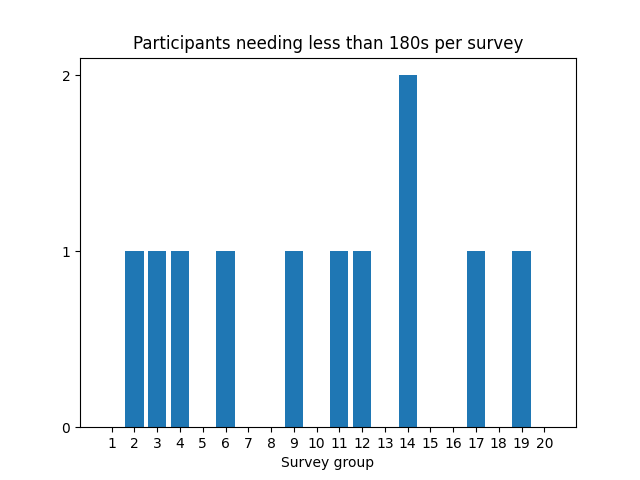
\includegraphics[width=0.75\textwidth]{img/survey_time_less_than_180.png}
		\caption{Amount of participants per survey sheet that required less than 3 minutes to complete the survey}
		\label{fig:survey_time_less_than_180}
	\end{figure}
	
	You can find an overview over the familiarity of the participants with Java in Figure \ref{fig:survey_java_familiarity_pie}.
	
	\begin{figure}[t]
		\centering
		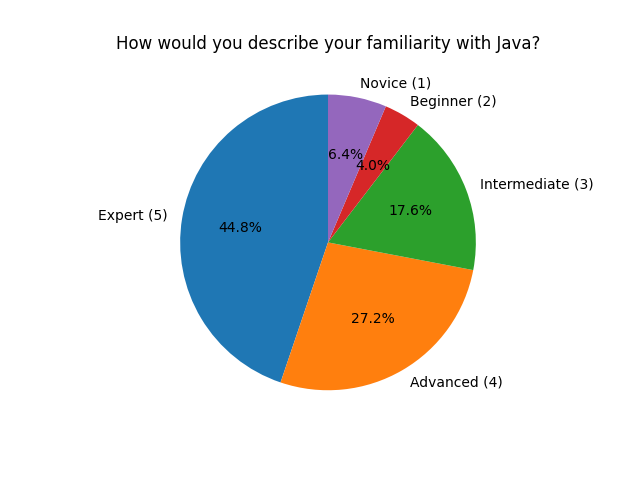
\includegraphics[width=\textwidth]{img/survey_java_familiarity_pie.png}
		\caption{Familiarity of survey participants with Java}
		\label{fig:survey_java_familiarity_pie}
	\end{figure}
	
	You can find an overview of the ratings for each RDH for all stratas combined in Figure \ref{fig:survey_ratings_violin_all}.
	
	\begin{figure}[t]
		\centering
		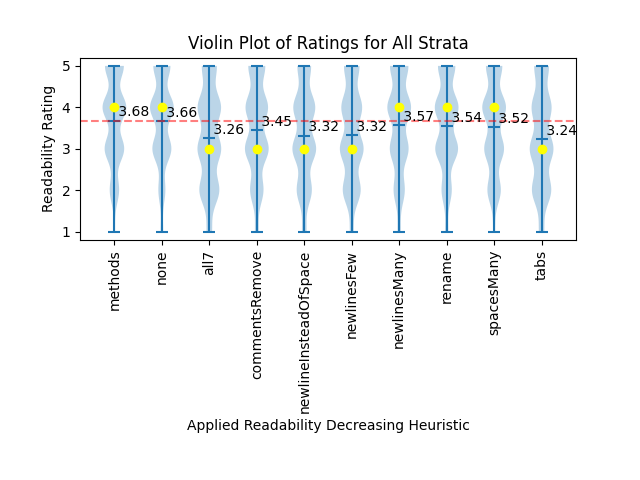
\includegraphics[width=\textwidth]{img/survey_ratings_violin_all.png}
		\caption{Violin plot of the survey ratings for each RDH and all stratas}
		\label{fig:survey_ratings_violin_all}
	\end{figure}
	
	We evaluated whether the deviation in the ratings between the various RDHs has statistical significance. We therefore used the Mann-Whitney-U-Test comparing the ratings for all snippets for a RDH against the corresponding none snippets. You can find the results of this in Table \ref{tab:survey_statistical_evidence}.
	
	Our results suggest, that doing no modification (none) is not different from the original methods. The difference here might as well come from a random variation with a probability of 92\%. When we compare the RDHs against the none methods we can be sure, that the ratings of all but newlines many and rename are actually statistically different from the ratings of none. This confirms that the readability decreasing heuristics are actually working in the sense that they decrease the readability of the given input methods.
	
	\begin{table}[h]
		\centering
		\begin{tabular}{lccc}
			\toprule
			\textbf{Condition} & \textbf{P-value} & \textbf{Reject} \\
			\midrule
			None - Methods & 0.9224 & False \\
			None - Newlines Few & $5.23 \times 10^{-6}$ & True \\
			None - Spaces Many & 0.0407 & True \\
			None - Newlines Many & 0.3006 & False \\
			None - Comments Remove & 0.00364 & True \\
			None - Rename & 0.099 & False \\
			None - Newline Instead Of Space & $4.57 \times 10^{-6}$ & True \\
			None - Tabs & $3.06 \times 10^{-8}$ & True \\
			None - All7 & $1.80 \times 10^{-7}$ & True \\
			\bottomrule
		\end{tabular}
		\caption{Mann-Whitney U Test Results of none against each RDH. If the p-value is smaller or equal to 0.05 the null-hypothesis is rejected confirming, that the ratings are actually different and not just a random variation. TODO: Update data}
		\label{tab:survey_statistical_evidence}
	\end{table}


\subsection{Model training results} \label{Model training results}
	You can find the training, evaluation and fine-tuning results in table \ref{tab:dataset_performance}.
	
	\begin{table}[h]
		\centering
		\begin{tabular}{|c|c|c|c|c|c|c|c|}
			\hline
			\textbf{Train} & \textbf{Eval} & \textbf{Acc} & \textbf{Prec} & \textbf{Rec} & \textbf{AUC} & \textbf{F1} & \textbf{MCC} \\
			\hline
			\textbf{Krod} 		& \textbf{Krod} 	& 0.918 & 0.923 & 0.913 & 0.918 & 0.917 & 0.836 \\
			\textbf{Krod} 		& \textbf{All}  	& 0.619 & 0.636 & 0.636 & 0.636 & 0.636 & 0.236 \\
			\textbf{All} 		& \textbf{Krod} 	& 0.538 & 0.526 & 0.778 & 0.652 & 0.628 & 0.087 \\
			\textbf{All}  		& \textbf{All}  	& 0.847 & 0.877 & 0.823 & 0.850 & 0.837 & 0.704 \\
			
			\textbf{Krod-FT-All}& \textbf{All}  	& 0.804 & 0.840 & 0.738 & 0.789 & 0.772 & 0.600 \\
			\textbf{Krod210}  	& \textbf{Krod210}  & 0.809 & 0.827 & 0.776 & 0.802 & 0.789 & 0.609 \\
			\hline
		\end{tabular}
		\caption{Performance of different dataset configurations for the same model. FT = Fine-Tuning}
		\label{tab:dataset_performance}
	\end{table}
	
	When training the towards model on the Krod dataset and evaluating it on it using 10-fold cross validation, we get an average accuracy score of 91.8\%. However, when we evaluate the trained model on the combined dataset used in the towards paper, we get an accuracy of only 61.9\%. We can conclude a couple of things from this:
	
	The towards model works well for our new dataset. However, the readability retrieved using the all dataset is different from the readability using our approach. Otherwise, the scores for all-krod and krod-all would be similar to the all-all score. This suggests, that our dataset is not suitable for general readability classification, but we might have found a subproblem. However, adding more readability decreasing features and adding well-designed data augmentation might overcome this limitation.
	
	When we compare the accuracy scores for all-krod and krod-all we get another interesting finding: While the model trained on the krod dataset is able to classify readabilty to some extend, this does not hold the other way around, as 53.8\% is almost a random classifier. This suggests, that fine-tuning a model trained on the krod dataset using the all dataset might score better results than the original model proposed in the towards paper.
	
	To verify that the model works correctly and as a baseline comparison score we also added the all-all case. Here we achieve the same accuracy as \citeauthor{mi2022towards}, which suggests that our model is implemented in the same way as theirs.
	
	We tried to do fine-tuning using the all dataset by freezing different layers of the model trained on the krod dataset. The best we could come up with was when freezing the input layers as well as the first convolution and pooling layer of all encoders. However, the performance of this fine-tuned model was still worse than the baseline model. This is in direct contrast to our previous suggestion, that fine-tuning in this way might score better results. One explanation for this might be, that the model is to small to deal with the now larger amount of data. Introducing more or bigger layers, so that the model can memorize more features internally might overcome this problem. However, this is not part of this work, where we soely deal with creating a new dataset.
	
	We also trained the model with a random sample of 210 datapoints to get a initial insight of what a change in the training size might accomplish. As we can see, the model has similar metrics as the all-all model. When we now compare the stats, for example the accuracy of the krod-krod against the all-all model, we can see, that an improvement of about 8\% might be possible with a larger dataset. This suggests the importance of finding new ways of data generation for readability classification.

	% Study evaluation
	% Assumption 1 - RQ1
	The readability ratings of code snippets mined from Github are not very accurate. Therefore the well readable assumption TODO only holds for certain clusters of code snippets: TODO. For clusters that can be labeled with X or Y this assumption does not hold. Therefore we labeled the mined code depending on the cluster they where grouped in as you can see in Table TODO. While the rating does not hold for each and every snippet within such a cluster it is a good estimation on average. This should be sufficient to train a readability classifier.
	
	% Assumption 2 - RQ2
	The badly readable assumption holds. Especially the heuristics X Y and Z decrease the readability by a significant extend. We estimate the readability decrease for a certain probability of a certain type as can be seen in table TODO. We therefore calculate the readability of a new snippet by taking the original readability score and decreasing the readability percent depending on the probability of such a refactoring beeing applied.	In Table TODO you can see how can to which extend we combined certain manually selected probabilities and how we then calculated the new readability score.
	
	% Model evaluation
	% Variant 1: More data
	When we compare the model of TOWARDS trained with the old dataset we can reproduce the results described in their paper. Once we add our own dataset we achieve an accuracy improvement of TODO. You can find a detailed comparison in Figure TODO.
	
	% Variant 2 & 3
	When we scale up the architecture by increasing XY we can achieve an even higher accuracy of TODO when using the new training data. However, with the old dataset only the results are worse. This suggests that the new fits the new larger dataset better while the architecture of TOWARDS was built for small datasets.
	% TODO: Method name fitting?
	% TODO: Encoding of tabs?
	
	% Dataset evaluation
	By combining the results of the study and model evaluation we can answer the third research question: The rating of our automatic dataset generation approach is not as accurate as letting multiple users rate a certain code snippet. However, being able to fully automate the dataset generation approach and the vast amount of data generated that way makes up for this. The larger dataset improves the performance, especially of our new adjusted model by a significant extent of TODO. Therefore we conclude, that our new dataset and it's generation approach is suitable for training deep learning based code readability classifiers.
	
	\section{Discussion} \label{Discussion}
	% Approach Threads
	The biggest thread to our approach is the reliance on heuristics for the dataset generation. We can not show, that the labeled code snippets of our dataset actually fit the score we assigned them. This would require an manual evaluation of X code snippets by human annotators and is therefore not feasible. We can reduce the extent of this with our model results. 
	
	% Study Threads
	TODO: Copy from study paper
	
	% Model threads
	TODO: Copy from towards and newer model
		
	
	\section{Conclusions} \label{Conclusions}
	TODO: Add conclusion
	
	% Future work
	% Transformer
	The new dataset has another advantage that is not yet utilized in this work: For the first time there is a dataset with one well readable and a second one less readable code snippet that is functionally equivalent. This could be used to train a transformer on source code readability improvement. Such a transformer could take code as input and improve it's readability. Such a tool would probably be of high usability among programmers.
	
	% Languages
	A current restriction of the dataset is that it only works for java code. Another proposal for future work is therefore to overcome this restriction by extending the tool for other languages. This is not trivial as one has to adjust the readability decreasing heuristics to work with a different language. Furthermore a general tool that works for all languages will be very hard, if possible at all.
	
	% Survey
	In order to further improve the readability estimations for both, the well and the badly readable code, one could conduct more s. By separating the code snippets into more fine granular clusters and by getting a more accurate average score by asking more persons about readability of code within the same cluster one can increase the accuracy of label estimation. Such an improvement can then again improve the model predictions as it is learning from this data.
	
	% Syntax Tree
	As XY suggested another useful representation for code readability studies is the syntax tree representation of code. One could improve the performance of this model by adding another representation encoding extractor for java code that automatically extracts the abstract syntax tree of code. 
	
	%  Method name fitting
	A crucial aspect of code readability is naming. For the scope of methods, the most crucial part are methods names. Therefore one could improve this tool by adding a component that explicitly considers how well a method name fits its body.
	
	% Other representations
	Further research could also be to come up with another encoding that represents code in a different way.
	
	% Other model structure
	Another way to improve existing code readability classifiers could be to come up with a different structure for some layers or entire different models.
	
	% More heuristics
	The heuristics described in this work is only a part of the possible heuristics one could come up with. One could come up with more heuristics and evaluate them using user studies in order to further improve the variety of badly readable code. This might increase the number of internal features the model could learn which might again increase the tools accuracy.

	
	\backmatter
	
	\printbibliography
	
\end{document}

% TODO: Appendix
%Did at first not where to rate the code
%I was confused about the textfield for the comments, because I only remembered that we should rate the code snippets, not that we have to make comments. Since I was not able to navigate back to the task description I did not know what to do with them.
%Für einen Anfänger mit sehr wenig Java Erfahrung ist meines Erachtens der Code zu kompliziert
%In the first place, I didn't really understand what readability meant. But after slide 3 or 4 I understood, what this was about.
%I found it difficult to categorize the first examples because you don't know what's still to come. For example, what the least readable code is.
%What problems were there with the survey tool? If there were none, leave blank.
%6 Antworten
%Mobile is not easy to use because of the scrolling needed to complete the survey
%First I needed to figure out how this tool works and that the rating is done with the stars below. I thought I should write my rating as a comment in the comment field below. After number 20 I didn't know whether I could close the survey or not.
%I also thought that I should use the drop-down menu on the upper left.
%It is sometimes necessary to swipe horizontally to see all of the code, which is a bit inconvenient.
%Für einen Anfänger ist das Tool meiner Meinung nach nicht geeignet. Der Code ist zu verschachtelt und teilweise unverständlich
%After finishing the task, at least message should be shown.
%I didn't understand what the button at the top left meant, where you could select the programming language. There were too many fonts to choose. I also wasn't sure whether to write a comment or not. It wasn't described at the beginning.
%What improvements would you make to the survey? If none, leave blank.
%6 Antworten
%Maybe one sentence that one should use the stars for the rating, then it would be clear. Also the submit note after the last question could contain that one can close the survey now.
%I suggest to make the task description accessible during the rating
%Maybe the option to leave the survey, when clicking to submit.
%Mehr Hilfestellung zum Lesen des Codes. Mehr Beschreibung oder ein zusätliches Cheat Sheet mit Bedeutungen von Befehlen
%I think it's good idea to ask the participant at the beginning to explain what readability mean for him.
%I would leave out the buttons described above. I was missing a scrollbar at the bottom of the code-window. A conclusion page with a message like "Thank you for your participation", "You're Done!" or other further information was missing, too.
%Do you have any other feedback? If none, leave blank.
%4 Antworten
%There werde drop downs for the programming language, but choosing another language did not change anything. It was a bit confusing that (almost?) all code snippets had very long imports within the code, which made them badly readable
%I spent the most time understanding methods with complete Java import names. (org.foo.bar.ClassName).
%-
%GOOD LUCK

% TODO: Appendix 2
%newline:
%- 0.0  # Probability for no newline
%- 1.0  # Probability for one newline
%incTab:
%- 0.0  # Probability for no tab
%- 1.0  # Probability for one tab
%decTab:
%- 0.0  # Probability for no tab
%- 1.0  # Probability for one tab
%space:
%- 0.0  # Probability for no space
%- 1.0  # Probability for one space
%newLineInsteadOfSpace: 0
%spaceInsteadOfNewline: 0
%incTabInsteadOfDecTab: 0
%decTabInsteadOfIncTab: 0
%renameVariable: 0
%renameField: 0
%renameMethod: 0
%inlineMethod: 0
%removeComment: 0
%add0: 0
%insertBraces: 0
%starImport: 0
%inlineField: 0.2
%partiallyEvaluate: 0
